
% mn2esample.tex
%
% v2.1 released 22nd May 2002 (G. Hutton)
%
% The mnsample.tex file has been amended to highlight
% the proper use of LaTeX2e code with the class file
% and using natbib cross-referencing. These changes
% do not reflect the original paper by A. V. Raveendran.
%
% Previous versions of this sample document were
% compatible with the LaTeX 2.09 style file mn.sty
% v1.2 released 5th September 1994 (M. Reed)
% v1.1 released 18th July 1994
% v1.0 released 28th January 1994


\documentclass[useAMS,usenatbib]{mn2e}
\usepackage{graphicx}
\usepackage{float}
\usepackage{wasysym}
\usepackage{stmaryrd}
\usepackage{txfonts}
\usepackage{natbib}
\usepackage{color}
\usepackage{colortbl}
\usepackage{multirow}

% Journal Definitions
\def   \aj {{\rm {AJ}}}
\def   \araa {{\rm {ARA\&A}}}
\def   \apj {{\rm {ApJ}}}
\def   \icarus {{\rm {Icarus}}}
\def   \apjs {{\rm {ApJS}}}
\def   \apss {{\rm {Ap\&SS}}}
\def   \aap {{\rm {A\&A}}}
\def   \aapr {{\rm {A\&AR}}}
\def   \aaps {{\rm {A\&AS}}}
\def   \baas {{\rm {BAAS}}}
\def   \memras {{\rm {MmRAS}}}
\def   \mnras {{\rm {MNRAS}}}
\def   \prl {{\rm {Phys. Rev. Lett.}}}
\def   \jqsrt {{\rm {Journal of Quantitative Spectroscopy and Radiative Transfer}}}
\def   \apjl{\rm {ApJL}}
\def   \nat{\rm {Nat.}}


% If your system does not have the AMS fonts version 2.0 installed, then
% remove the useAMS option.
%
% useAMS allows you to obtain upright Greek characters.
% e.g. \umu, \upi etc.  See the section on "Upright Greek characters" in
% this guide for further information.
%
% If you are using AMS 2.0 fonts, bold math letters/symbols are available
% at a larger range of sizes for NFSS release 1 and 2 (using \boldmath or
% preferably \bmath).
%
% The usenatbib command allows the use of Patrick Daly's natbib.sty for
% cross-referencing.
%
% If you wish to typeset the paper in Times font (if you do not have the
% PostScript Type 1 Computer Modern fonts you will need to do this to get
% smoother fonts in a PDF file) then uncomment the next line
% \usepackage{Times}

%%%%% AUTHORS - PLACE YOUR OWN MACROS HERE %%%%%


%%%%%%%%%%%%%%%%%%%%%%%%%%%%%%%%%%%%%%%%%%%%%%%%

\title[Young protoplanetary discs]{Simulated Observations of Young Protoplanetary Discs}
%%authors arent splitting over 2 lines so rawlings is pushed off the edge
%\author[Tom Douglas, Paola Caselli, Et al.]{Tom Douglas$^{1}$\thanks{E-mail:
%pytd@leeds.ac.uk}, Paola Caselli$^{1}$, Aaron Boley$^{2}$, Richard Durisen$^{3}$, Tom Hartquist$^{1}$, %John Ilee$^{1}$, Jonathon Rawlings$^{4}$ \\
%$^{1}$School of Physics and Astronomy, University of Leeds, Leeds LS2 9JT, UK \\
%$^{2}$Department of Astronomy, University of Florida, 211 Bryant Space Center, PO Box 112055, USA\\
%$^{3}$Department of Astronomy, Indiana University, 727 East 3rd Street, Swain West 319, Bloomington, IN %47405, USA\\
%%$^{4}$Department of Physics & Astronomy, University College London, London WC1E 6BT, UK\\
%}

\author[T.~A.~Douglas et al.]
{\parbox{\textwidth}{Tom Douglas$^{1}$\thanks{E-mail: \texttt{pytd@leeds.ac.uk}},
Paola Caselli$^{1}$,
Aaron Boley$^{2}$,
Richard Durisen$^{3}$,
Tom Hartquist$^{1}$,
John Ilee$^{1}$ and
Jonathan Rawlings$^{4}$\\
\vspace{0.1cm}\\
{\small{\it$^{1}$School of Physics and Astronomy, University of Leeds, Leeds LS2 9JT, UK}} \\
{\small{\it$^{2}$Department of Astronomy, University of Florida, 211 Bryant Space Center, PO Box 112055, USA}}\\
{\small{\it$^{3}$Department of Astronomy, Indiana University, 727 East 3rd Street, Swain West 319, Bloomington, IN 47405, USA}}\\
{\small{\it$^{4}$Department of Physics \& Astronomy, University College London, London WC1E 6BT, UK}}\\}}


%{\parbox{\textwidth}{
%$^{1}$School of Physics and Astronomy, University of Leeds, Leeds LS2 9JT, UK \\
%$^{2}$Department of Astronomy, University of Florida, 211 Bryant Space Center, PO Box 112055, USA\\
%$^{3}$Department of Astronomy, Indiana University, 727 East 3rd Street, Swain West 319, Bloomington, IN %47405, USA\\
%$^{4}$Department of Physics & Astronomy, University College London, London WC1E 6BT, UK\\
%}}



\begin{document}

\date{Jan 2013}

\pagerange{\pageref{firstpage}--\pageref{lastpage}} \pubyear{2002}

\maketitle

\label{firstpage}

\begin{abstract}
The formation and earliest stages of protoplanetary discs are still lacking observational constraints. ALMA will soon revolutionise this field, so it is important to provide predictions and help the interpretation of future high sensitivity and high angular resolution observations. Here we present simulated ALMA observations based on radiative transfer modelling of a relatively massive (0.39 M$_{\odot}$) self-gravitating disc embedded in a 10\,M$_{\odot}$ dense core, with structure similar to the pre-stellar core L1544. We focus on simple species and conclude that OCS, C$^{17}$O, H$_2$CO and HCO$^+$ lines together allow for measurements of the disc structure and kinematics at all scales. 
\end{abstract}

\begin{keywords}
circumstellar matter -- infrared: stars.
\end{keywords}

\section{Introduction}

The formation and early evolution of protoplanetary discs around solar-type and low-mass protostars has little observational support, despite of the fast growing list of theoretical models on the dynamical evolution of star forming dense cores (e.g. Krasnopolsky et al. 2011; Machida et al. 2011; Braiding \& Wardle 2012; Joos et al. 2013). The reason for this is that young protostars are surrounded by thick envelopes and power energetic outflows. Thus, observations of the young discs, predicted to have sizes of about 100\,AU and masses as large as 10\% the original core mass (e.g. Joos et al. 2012), are challenging. The use of sensitive interferometers is needed to achieve high angular resolution and spatially/spectrally disentangle the various disc, envelope and outflow components as well to filter out the extended emission tracing envelope material. \newline

After the pioneer work of, e.g., Chandler et al. (1995), Brown et al. (2000), Looney et al. (2000), recent interferometric observations have discovered compact embedded discs in a sample of Class 0 (Andr\'e et al. 2000) sources, finding masses between 0.4 and  $>$1 M$_{\odot}$ (J\o rgensen et al. 2007, 2009; Enoch et al. 2011). A 130\,AU disc was discovered toward a Class 0 source in Perseus, using Jansky Very Large Array (JVLA) observations of NH$_3$ (Choi et al. 2007). Pineda et al. (2012) observed methyl formate with the Atacama Millimetre and millimetre Array (ALMA) and found evidence of rotation toward one of the proto-binary Class 0 sources embedded in IRAS 16293-2422. These observations are consistent with an almost edge-on disc. Persson et al. (2012) observed H$_2^{18}$O with ALMA toward the same source and found evidence of relatively large ($\ga$100\,K) excitation temperatures, as well as a HDO/H$_2$O abundance ratio close to that measured on Earth's oceans and Jupiter-family comets (Hartogh et al. 2011). Zapata et al. (2013) used ALMA to observe a disc of size $\sim$50$\,$AU in the other Class 0 source in IRAS 16293-2422 and detected infall towards this disc as inverse P-Cygni profiles in HCN and CH$_3$OH. When ALMA will be completed, it will be finally possible to spatially resolve these young discs and, for the first time, put stringent constraints on theoretical models. As full-operational ALMA is fast approaching, it is important to provide observational predictions based on dynamical models of young protoplanetary discs. \newline 

Simulated observations of gravitationally unstable discs have already been performed to study the continuum emission and measure the structure and possible fragmentation (Cossins et al. 2010; Ruge et al. 2013). Molecular line emission from massive discs has been simulated by Krumholz et al. (2007), assuming local thermodynamic equilibrium (LTE). In this paper, we focus on the self-gravitating discs of Boley \& Durisen (2008), where episodic heating induced by spiral shocks is present. This may be a good representation of the earliest phases of protoplanetary discs and an alternative to the young ``static'' discs studied by, e.g., Visser et al. (2009, 2011). As shown by Ilee et al. (2011; hereafter I2011), the spiral shocks cause desorption of volatiles from dust icy mantles and trigger gas-phase chemical reactions with activation energies, too high to occur at lower temperatures. These processes produce clear chemical signatures of the disc dynamics. With the use of 3D radiative transfer modelling, we perform simulated ALMA observations of the disc studied by I2011 and identify the best tracers of the physical structure of self-gravitating discs. The physical, chemical and radiative transfer models are described in Sect.\,\ref{sec:description_model}. Radiative transfer results are in Sect.\,\ref{sec:model_results}, while ALMA simulated observations are in Sect.\,\ref{sec:alma_predictions}. Discussions and conclusions can be found in Sect.\,\ref{sec:discussion}. 

\section{Description of the Model} \label{sec:description_model}

\subsection{Physical and chemical structure} \label{subsec:physical_structure}


The physical model used to simulate the emission from a young protoplanetary disc is a hybrid model obtained from embedding a gravitationally unstable protoplanetary disc  within a dense core with characteristics similar to the well-studied pre-stellar core L1544, (Keto \& Caselli 2010; hereafter KC2010). The KC2010 model follows the dynamical, chemical and thermal evolution of a contracting Bonnor-Ebert sphere (Bonnor 1956; Ebert 1957) with total mass of 10\,M$_{\odot}$, until it reaches the density, temperature and velocity profiles which best match observations. The pre-stellar core model adopted here contains slight modifications due to the inclusion of oxygen cooling in the outer regions of the cloud, where CO is mostly photodissociated (Caselli et al. 2012; Keto et al. in preparation), and it is shown in Fig.\,\ref{fig:l1544_model}. \newline

\begin{figure}
 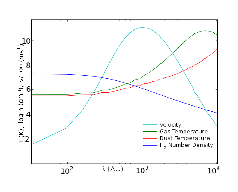
\includegraphics[width=84mm]{Figures/model/L1544model_used_legend_small.eps}
 \caption{The spherically symmetric model of the pre-stellar core L1544 used as the envelope of the young protoplanetary disc in the hybrid model. Showing temperature (green) and dust (red) temperature in kelvin, log number density (blue) in cm$^{-3}$ and inward velocity / 100 (cyan) in m$\,$s$^{-1}$. Adapted from KC2010 and Keto et al. (2013, in preparation).}
 \label{fig:l1544_model}
\end{figure}


\begin{figure*}
 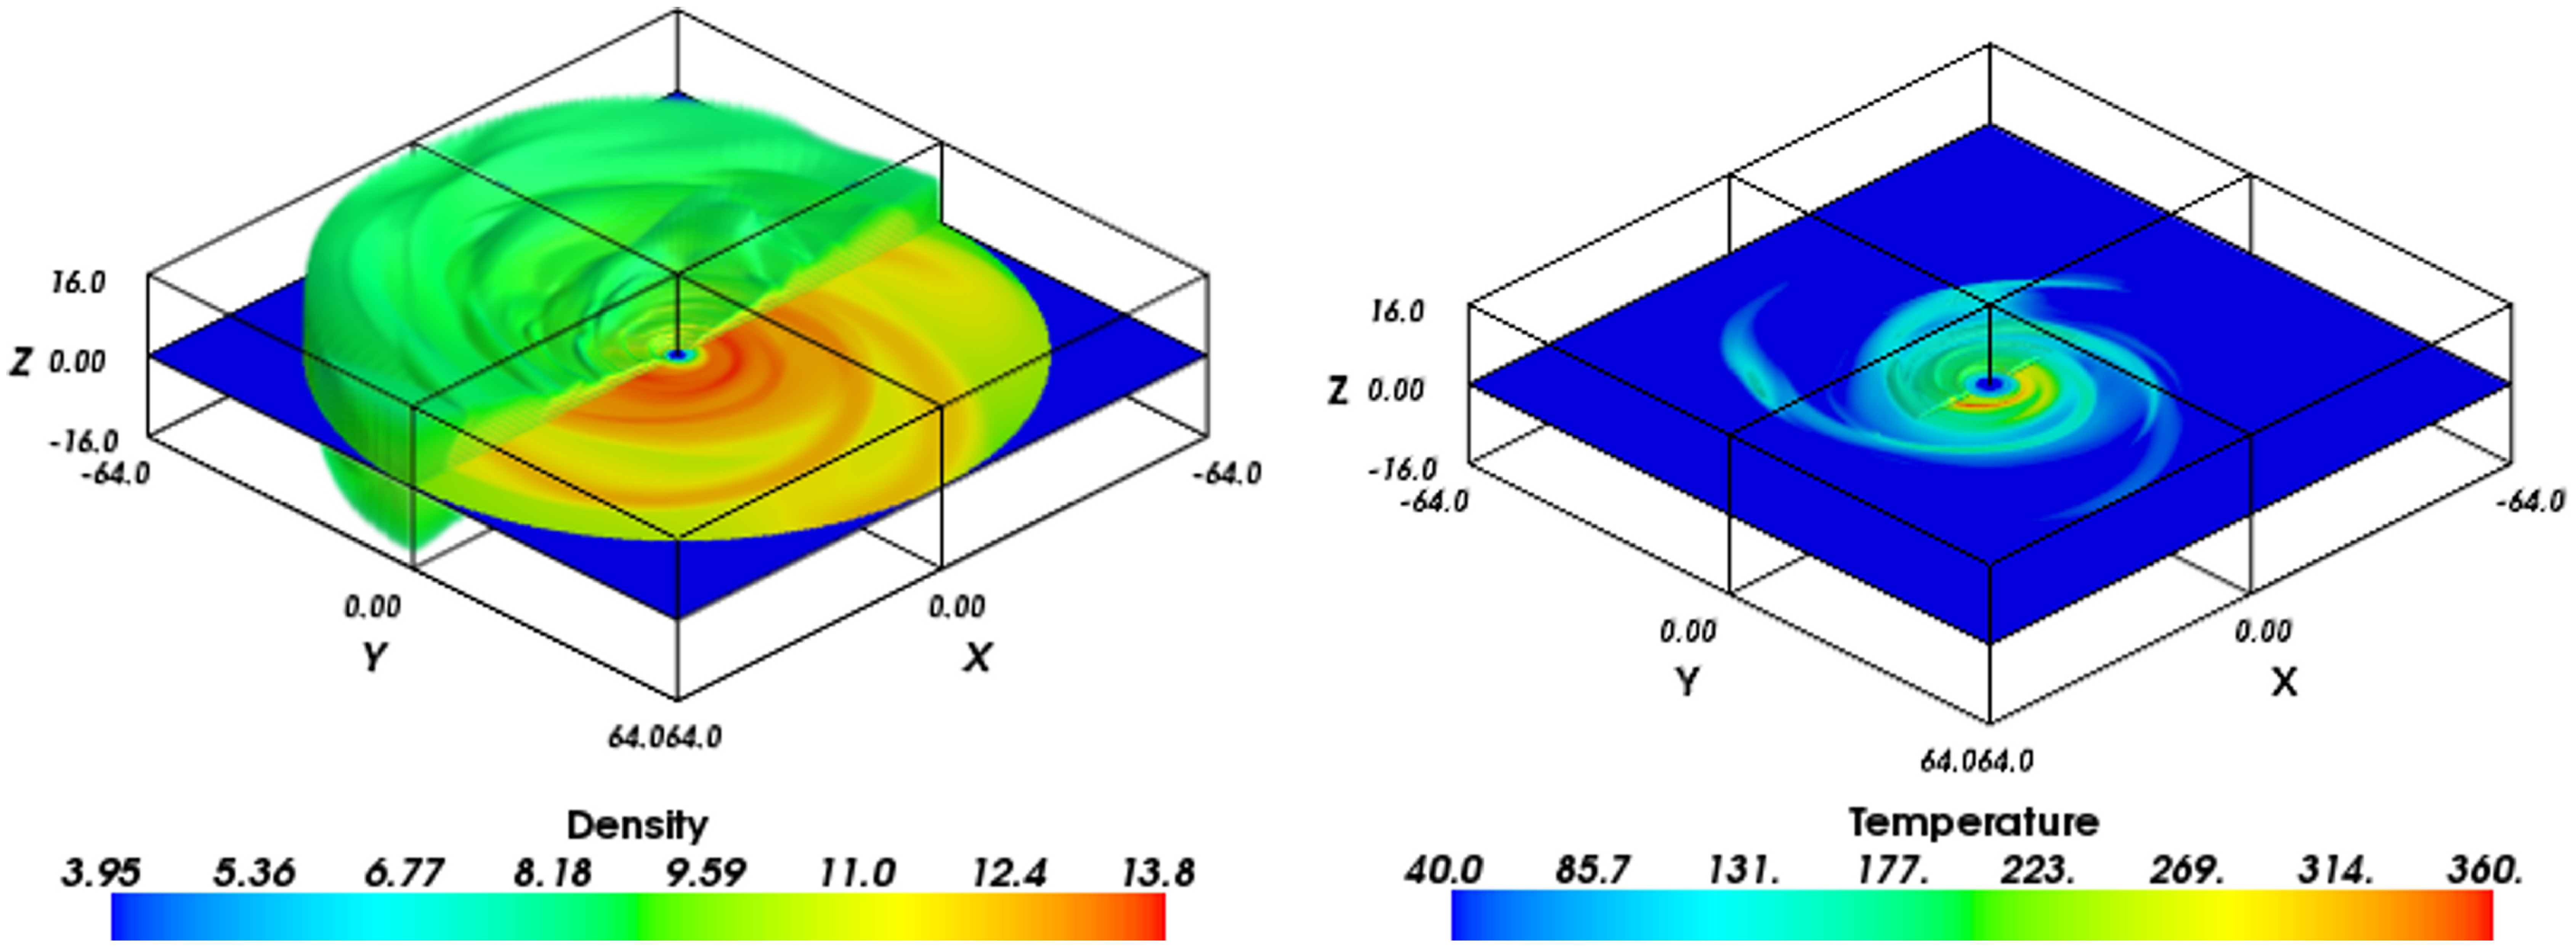
\includegraphics[width=168mm]{Figures/model/rhoT6.eps}
 \caption{{\bf Left:} A 3D plot of log number density (cm$^{-3}$) showing the spiral structure in the xy plane and scale height of the disc. {\bf Right:} The 3D temperature structure of the disc; regions cooler than 40 degrees are not shown in 3D, highlighting the narrow central region containing hot material.}
 \label{rhoT} 
\end{figure*}

\begin{figure*}
 \includegraphics[width=168mm]{Figures/model/columnDensities2.eps}
 \caption{Column densities of OCS, H$_2$CO,HCO$^+$ and CO used in the disc model. Figure adapted from I2011}
 \label{Chemistry} 
\end{figure*}

\begin{figure}
 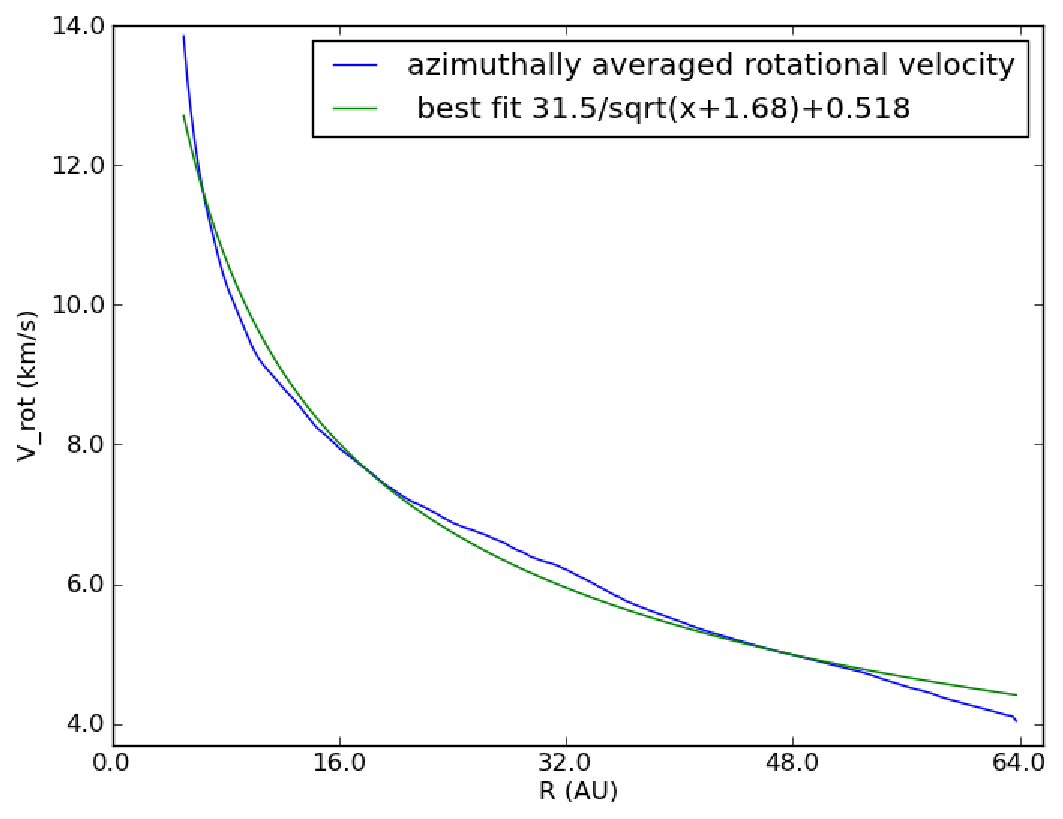
\includegraphics[width=84mm]{Figures/model/rotational_velocities.eps}
 \caption{Azimuthaly averaged rotational velocity in the disc mid-plane with best fit curve}
 \label{velocity}
\end{figure}


The pre-stellar core structure is maintained down to a radius of 80\,AU, within which the young protoplanetary disc has been plugged in. The disc structure is derived by the hydrodynamic model of Boley (2007) and Boley (2009). The particular model considered here (as well as in I2011) is a 0.39$\,\rm{M}_\odot$ self-gravitating disc featuring prominent spiral arms. H$_2$ number densities in the disc range from 10$^{4}$-10$^{13}\,\rm{cm}^{-3}$, and temperatures range from 30-400 K (figure \ref{rhoT}). The dust and gas temperatures in the disc are assumed to be in equilibrium. The underlying model is sampled as a regular grid of size 256$\times$256$\times$64 with spatial resolution of 0.5$\,$AU in x, y and z. The gas/dust mass ratio was assumed to be 1/100 throughout both sections model and the opacities were adopted from Ossenkops and Henning (1994) and refer to dust grains with thick icy mantles and 10$^6$ yr coagulation history.\newline

Chemical abundances in the disc were taken from I2011 who followed gas-grain chemical processes during the dynamical evolution of the disc. The abundances of 125 species related by 1334 reactions were calculated through the time evolution of the disc. These abundances were interpolated onto a 51$^3$ grid covering the disc with cells of size 2.2$\times$2.2$\times$0.22$\,$AU.  From I2011 we selected the four species which appear to trace different regions of the disc: the inner 20\,AU (OCS), the inner 40\,AU (H$_2$CO),  the region between $\simeq$40 and 60\,AU (HCO$^+$) and one which traces the entirety of the disc (C$^{17}$O) (see figure \ref{Chemistry}, the abundance model used for C$^{17}$O was the CO model reduced by a factor of 1792, the ratio of $^{16}$O to $^{17}$O in the local ISM, Wilson \& Rood 1994). As explained by I2011,  H$_2$CO and OCS mostly probe the central warm regions, where icy mantles evaporate, whereas HCO$^+$ preferentially traces the outer spiral pattern as in the central region it is destroyed by water molecules and transformed into H$_3$O$^+$ and CO. The simple chemistry in the KC2010 model, adopted here as the envelope of the protoplanetary disc, does not provide detailed abundances of molecular species (besides CO and H$_2$O, see also Caselli et al. 2012). As discussed in the result section (Sec.\,\ref{sec:model_results}), rough guesses have been made based on values measured toward similar objects. The molecular data used is from the lamda database (Sch\"oier et al. (2005) http://home.strw.leidenuniv.nl/$\sim$moldata/).


\subsection{The radiative transfer code} \label{subsec:radiative_transfer_code}
%-describe the RT used (LIME) 
%-describe the RT used (LIME) 
The radiative transfer program used is LIME (Brinch \& Hogerheijde 2010),which  calculates line intensities based on a weighted sample of randomly chosen points in a continuous 3D model. The method of selecting these points is given in the grid-construction section (section \ref{gridding}). At each of these points, the density of the main collision partner (H$_2$), gas and dust temperatures, velocity, molecular abundances and turbulent velocity are specified. These points are then smoothed by Lloyd's algorithm (Lloyd 1982) in order to minimise the variation in distance between points whilst keeping the same underlying distribution. These points are then connected by Delaunay triangulation \footnote{In three dimensions this means that if four points are connected into a tetrahedron, the sphere circumscribing these four points contains no other points. It can be shown that this connection is unique for a given set of points.} and it is down these paths that photon propagation is restricted (figure \ref{grid}). The level populations of the selected molecules are calculated at each of these points from collisional and radiative (de)excitation and the local radiation field is calculated. This is repeated 20 times with the populations of each level converging towards a single value. This number of iterations is sufficient for the signal to noise ratio of the level populations (as defined in Brinch \&Hogerheijde 2010) to exceed 1000 in 99\% of the points, ensuring that the simulation has converged on a stable level population. After 20 iterations the model is ray-traced in order to produce synthetic brightness maps. In order to minimise the artifacts in the output images, resulting from the grid construction, the average of ten separate runs was taken (figure \ref{averages}).


\begin{figure}
 \includegraphics[width=84mm]{Figures/model/grid.eps}%Lime_grid3.eps
 \caption{A plot of the points selected by the griding process and the paths down which photons can propagate overlaid on the density distribution (in m$^{-3}$, as used in LIME). The points are more concentrated at small radii and in the densest regions.}
 \label{grid}
\end{figure}

\section{Model Results} \label{sec:model_results}

Simulations are limited to molecules for which we have abundances in both the disc and envelope, and also have calculated Einstein and collisional coefficients. We focus on the frequency range available with ALMA, with particular attention to band 7, which offers the best trade off between resolution and sensitivity. The results presented in this section are limited to those lines which show detectable emission/absorption which can be used to trace either spiral structure or rotation.\newline

We considered C$^{17}$O 3-2 at 337.1GHz with an upper energy level of $E_u$=32.3K, HCO$^+$ 3-2 at 267GHZ and $E_u$=25.7K, OCS 26-25 at 316GHz and $E_u$=205K and H$_2$CO $4_{04}$-3$_{03}$ at 290GHz and $E_u$=34.9K. Other molecules simulated but not shown include HCN, HNC, HNO, HCS$^+$ and CS.\newline

To simulate observations, the model was placed at roughly the distance of nearby low-mass star forming regions (100$\,$pc) and the disc is inclined at 30$^\circ$ to edge on. From these simulated observations, integrated intensity, intensity weighted velocity and position velocity diagrams through the centre of the model were created.
We focus on the frequency range available with ALMA, with particular attention to band 7, which offers the best trade off between resolution and sensitivity.
(Note the integrated intensity and intensity weighted velocity maps (figures \ref{sim_all} and \ref{mom0_maps}) were created by integrating between -12.5 to -0.5 km$\,$s$^{-1}$ and +0.5 to +12.5 km$\,$s$^{-1}$ to avoid being dominated by the contribution from the envelope, this can be seen in some PV diagrams  (figure \ref{pvs}) as the strong absorption feature at all positions around zero velocity, moment 1 maps are shown with a cut-off of 3$\sigma$ as described in section \ref{sec:alma_predictions})\newline

\begin{figure}
 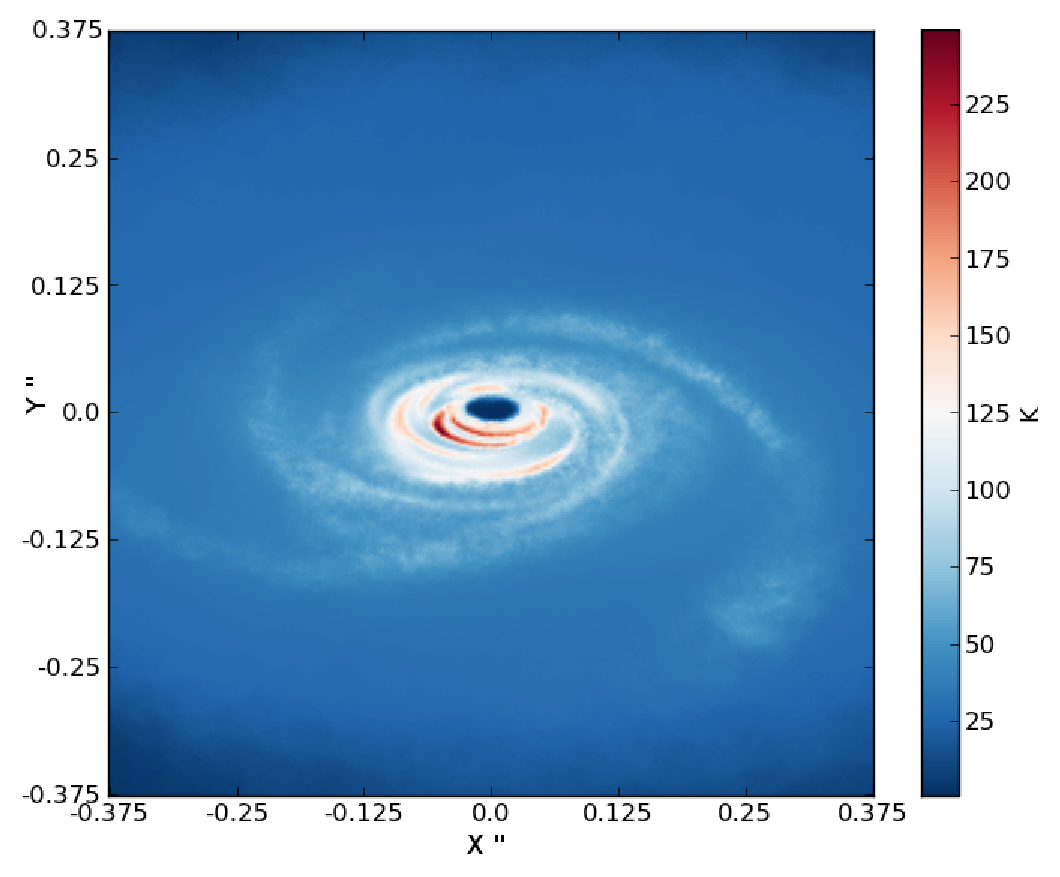
\includegraphics[width=84mm]{Figures/sim/continuum.eps}
 \caption{{\bf Left:}A 300$\,$GHz continuum image of the model, created from the average of ten LIME runs. {\bf Right:} the output of a single radiative transfer simulation, with artifacts due to finite griding.}
 \label{averages}
\end{figure}

\begin{figure*}
 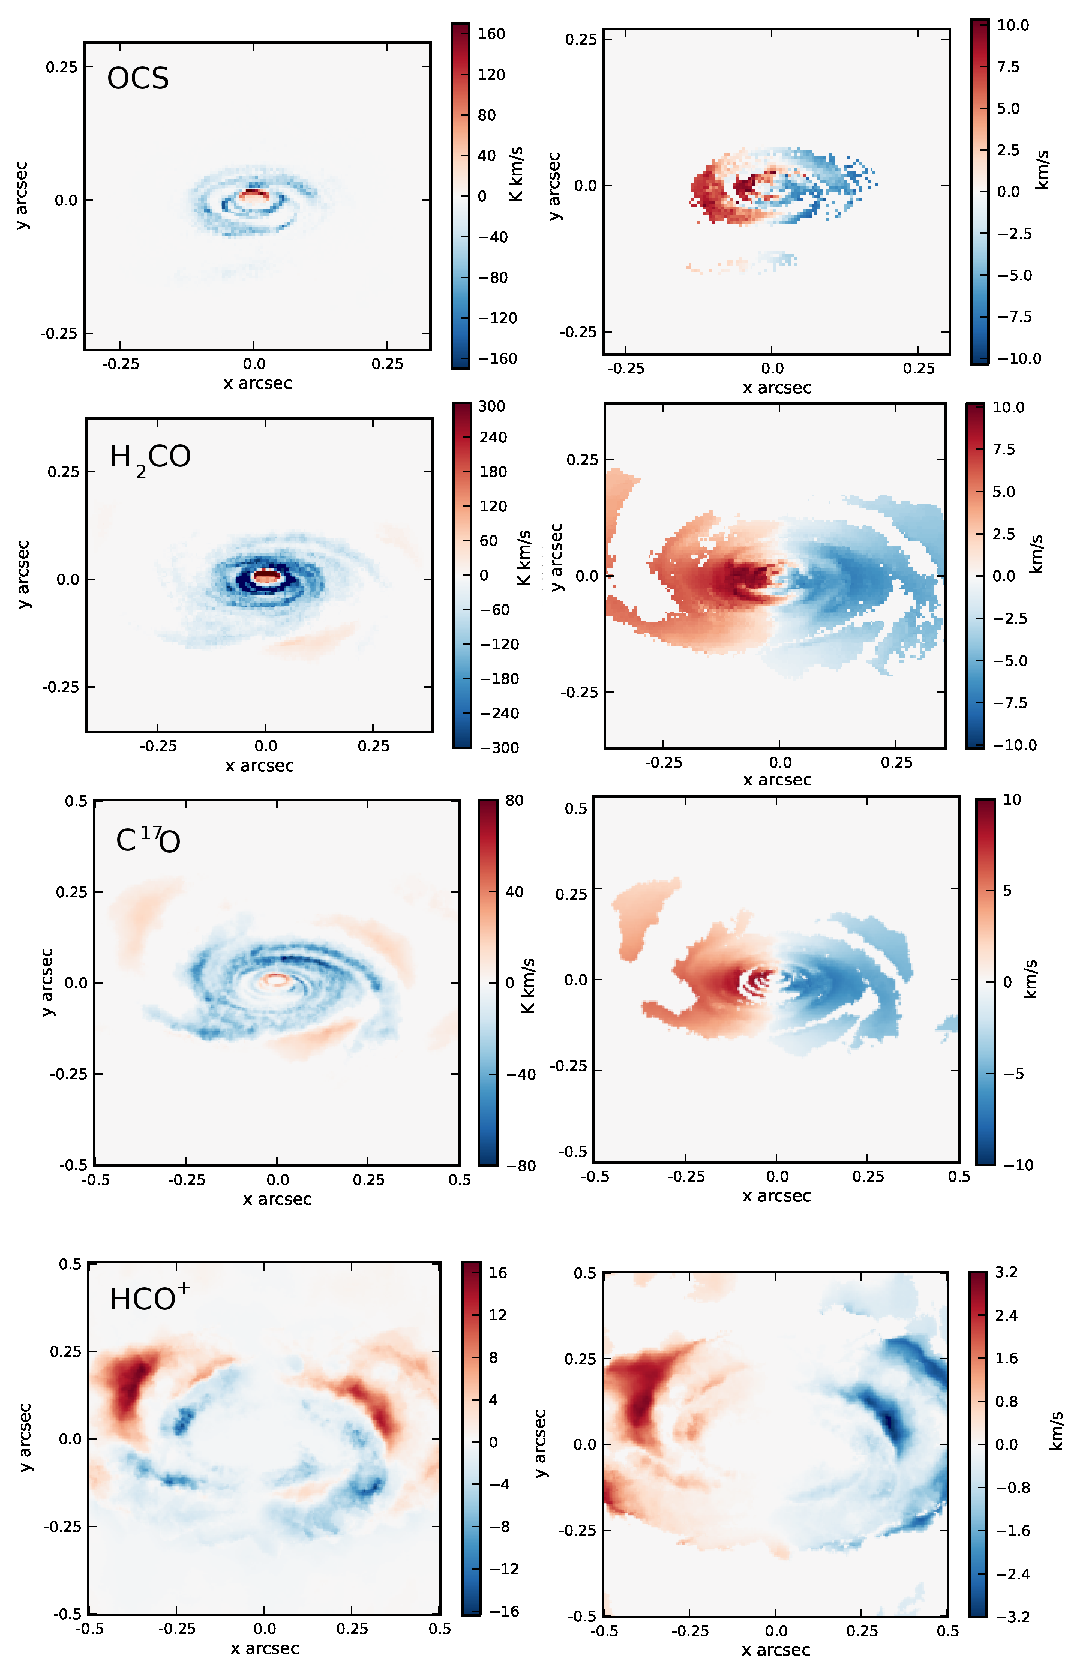
\includegraphics[width=150mm]{Figures/sim/imageALL_30deg_all.eps}
 \caption{{\bf Left:}Continuum subtracted integrated intensity maps, {\bf Right:} Intensity weighted velocity maps. The spiral structure in different regions of the disc is highlighted by looking at different molecular lines. From top to bottom the lines displayed are: OCS 26$\rightarrow$25, H$_2$CO 4$_{04}$$\rightarrow$3$_{03}$, C$^{17}$O 3$\rightarrow$2 and HCO$^+$ 3$\rightarrow$2. All maps are integrated over -12.5 to -0.5 and 0.5 to 12.5 km$\,$s$^{-1}$ in order to avoid the envelope contribution.}
 \label{sim_all}
\end{figure*}


OCS traces only the innermost 20$\,$AU of the disc and can be used to examine the central regions (figure \ref{sim_all}). As OCS is not seen in outflows (e.g. Stanke 07, Van der Tak 03) it can be used to view rotation of the central part of the disc without risk of contamination from emission from shocked material. The OCS line, which has the highest upper energy level among the selected transitions, traces the hottest and densest regions of the disc. As a result, the innermost spiral structure is best seen in OCS (26 - 25), as shown in figure \ref{sim_all}. The majority of the OCS line is visible in absorption against the bright continuum emission from the disc mid-plane. The exception to this is towards the centre of the disc where the hole in the hot, dense mid-plane means that there is little continuum to be absorbed.\newline

The abundance of the H$_2$CO molecule is typical of the majority of the molecules simulated in I2011 in that it traces the spiral structure of the inner $\sim$40$\,$AU of the disc. The spiral structure of the disc can be seen clearly in the integrated intensity map and its rotation of detected out to larger radii than is possible with the OCS (figure \ref{sim_all}). As with the OCS line, the majority of the H$_2$CO 4$_{04}$-3$_{03}$ line is seen in absorption against the disc mid-plane continuum with the central region seen in emission. Unlike the OCS however, the H$_2$CO extends out to large enough radii to be present in the voids between spiral arms. In these regions the H$_2$CO line can be seen in emission, this can be seen most clearly in the H$_2$CO channel map (figure \ref{h2co_chanmap}).\newline

The fractional abundance of C$^{17}$O is constant at 2$\times$10$^{-8}$ across the disc, meaning the C$^{17}$O line is the most accurate in reproducing the physical structure of the disc. Like H$_2$CO, C$^{17}$O shows emission in voids between spiral arms. The C$^{17}$O line is visible from inner edge of the disc to its outer edge. Like OCS, C$^{17}$O is not seen in outflows (e.g. Yildiz et al. 2012) and so rotation seen in C$^{17}$O lines should only be due to rotation from the disc and not contamination from outflows.\newline

HCO$^+$ in unique in the molecules simulated in I2011 in that it traces only the outer regions of the disc, and so can be used to look at the extended velocity and physical structure. In figure \ref{sim_all} we can see that the HCO$^+$ line shows the outer edges of the spiral arms in absorption, but also shows emission from the diffuse gas further out in the disc. This allows the velocity structure of the disc measured out to larger radii. This allows constraints to be placed on the rotation of the disc out to larger radii than other molecules. 


\section{ALMA Predictions} \label{sec:alma_predictions}

In order to make predictions on the observability of the synthetic brightness maps CASA (common astronomy software applications) was used to simulate their observation with the completed ALMA in configuration 26 of 28, giving a beam size of between 0.02 and 0.03 arcseconds. As the weakest lines studied in the model are of the order of 0.1-0.2$\,$mJy$\,$beam$^{-1}$ at this resolution, sensitivities of the order of 0.02$\,$mJy$\,$beam$^{-1}$ are required. This requires around 6 hours of integration time. The exact sensitivities are give in table \ref{sigmas}.
\begin{table}
 \centering
 \begin{minipage}{80mm}
   \caption{Sensitivities of ALMA given 6 hours integration time with velocity resolution of $\sim$400$\,$ms$^{-1}$. As calculated by the ALMA on-line sensitivity calculator.}
   \label{sigmas}
   \begin{tabular}{c||c|c|c}
     \hline
     Species & Transition & Frequency & Sensitivity\\
     \hline
     C$^{17}$O & J=3$\rightarrow$2 & 337.06GHz & 0.0270$\,$mJy$\,$beam$^{-1}$ \\
     OCS & J=26$\rightarrow$25 & 316.15GHz & 0.0275$\,$mJy$\,$beam$^{-1}$ \\
     HCO$^+$ & J=3$\rightarrow$2 & 267.56GHz & 0.0176$\,$mJy$\,$beam$^{-1}$ \\
     H$_2$CO & 4$_{04}\rightarrow$3$_{03}$ & 290.62GHz & 0.0228$\,$mJy$\,$beam$^{-1}$ \\
     \hline
   \end{tabular}
 \end{minipage}
\end{table}
In order to clean the images which featured mainly absorption the sky model used was the output of the lime simulations with the continuum subtracted and then the image inverted. The simulated images were cleaned down to a 3$\sigma$ level with $\sigma$ given in table \ref{sigmas}.\newline

\begin{figure}
 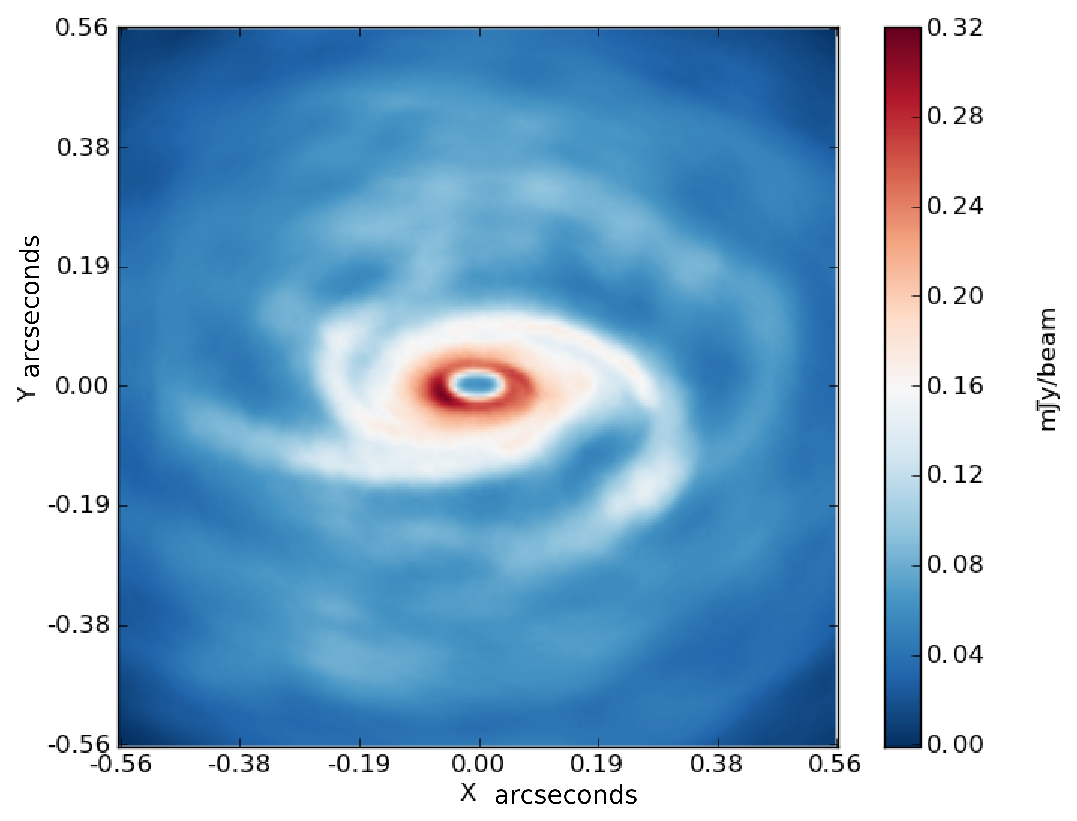
\includegraphics[width=84mm]{Figures/sim/casa_cont_337GHz.eps}

 \caption{Continuum emission at 337GHz simulated for ALMA most extended configuration}
 \label{continuum}
\end{figure}


\begin{figure*}
 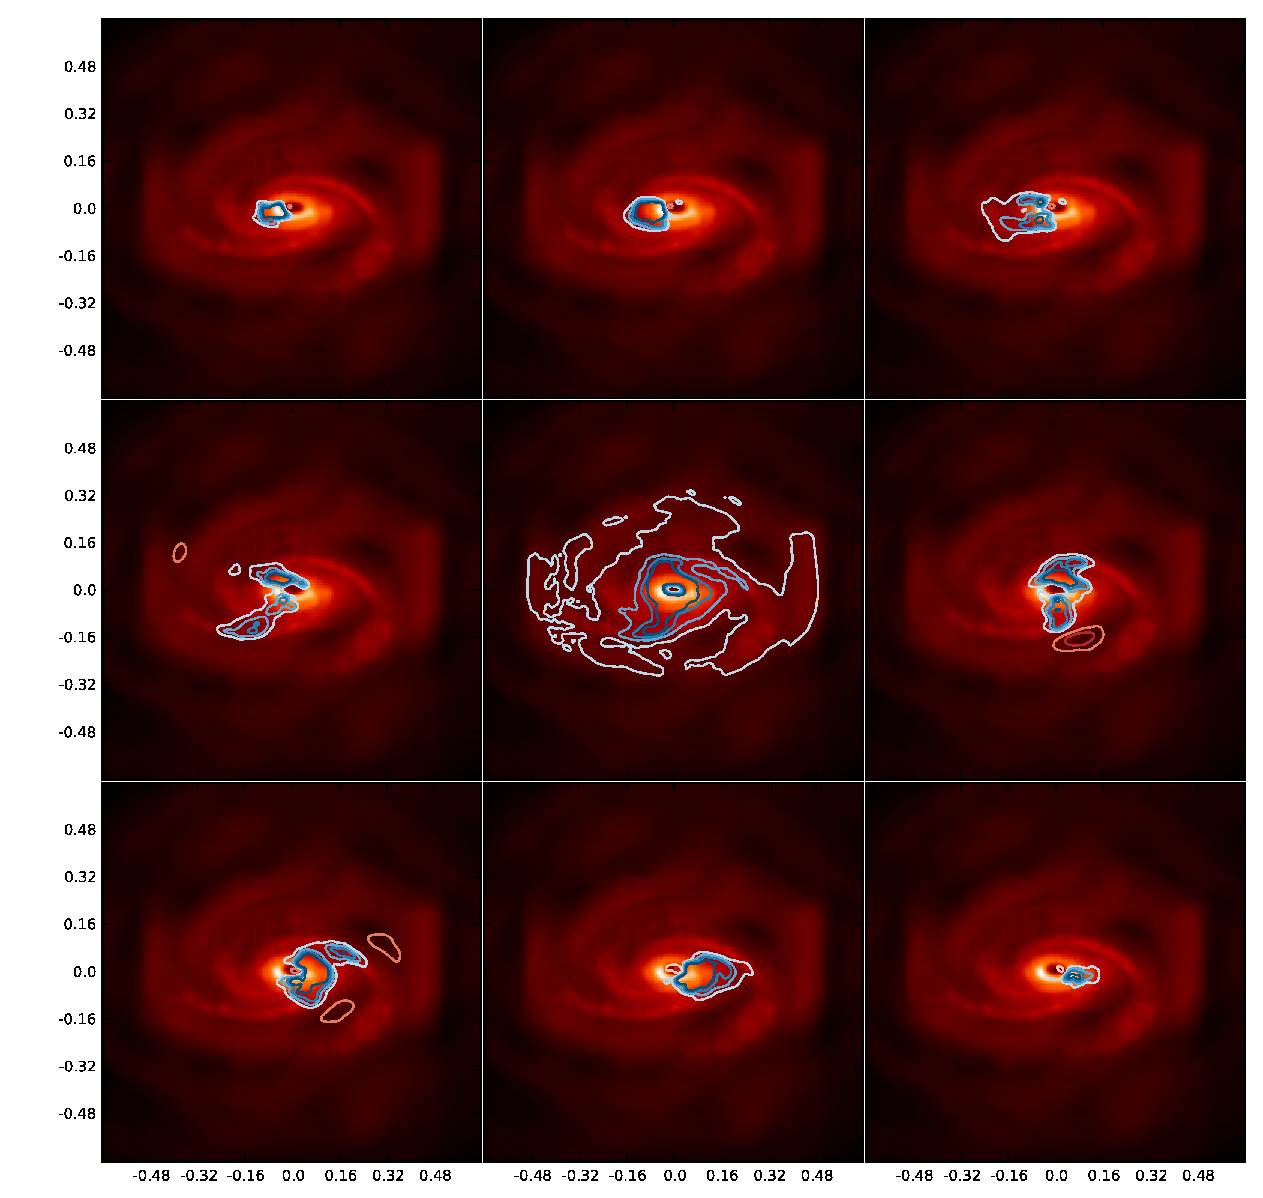
\includegraphics[width=168mm]{Figures/sim/channel_map-1.eps} 
 \caption{H$_2$CO 4$_{04}$-3$_{03}$ channel maps as simulated by CASA. H$_2$CO line in contours starting at 0.35 mJy$\,$beam$^{-1}\,$km$\,$s$^{-1}$ (absorption in blue, emission in red). Overlaid on the 1mm continuum emission. Each map integrates over 2.4 km$\,$s$^{-1}$ with the top left from -10.8 to -8.4 km$\,$s$^{-1}$ to the bottom left ranging from 8.4 to 10.8 km$\,$s$^{-1}$}
 \label{h2co_chanmap}
\end{figure*}

Figure \ref{h2co_chanmap} shows a channel map of the H$_2$CO 4$_{04}$-$3_{03}$ line overlaid on the 1$\,$mm continuum emission (figure \ref{continuum}). From this it can be seen that the absorption features trace the disc spiral structure whilst line emission emanates from gaps in the disc where there is less continuum to be absorbed.\newline


\begin{figure*}
 \includegraphics[width=168mm]{Figures/sim/casa_all_30deg_contSub_nums.eps}
 \caption{Integrated intensity maps for the simulated observations of:{\bf Top Left:} H$_2$CO 4$_{04}\rightarrow$3$_{03}$, {\bf Top Right:}C$^{17}$O 3$\rightarrow$2, {\bf Bottom Left:} OCS 26$\rightarrow$25 and {\bf Bottom Right:} HCO$^+$ 3$\rightarrow$2. contours start at 3$\sigma$ and increasing in intervals of 3$\sigma$ for each of the maps except the H$_2$CO which starts at 5$\sigma$ and increases in intervals of 5$\sigma$. Emission is in red contours, absorption in blue. The numbers refer to the spectra shown in figure \ref{spectra}.}
\label{mom0_maps}
\end{figure*}

Figure \ref{mom0_maps} shows the simulated integrated intensity maps, which demonstrate how different species allow observations to trace different regions of the disc, from OCS tracing the innermost regions to HCO$^+$ showing the outer regions which are less bright in the continuum. ALMA has enough resolution and sensitivity to see spiral structure clearly in continuum emission but also in CO isotopologues and marginally in H$_2$CO.\newline


\begin{figure*}
 \includegraphics[width=198mm]{Figures/sim/casa_all_30deg_PV_rotCurve.eps}
 \caption{Position velocity diagrams for each of the species simulated with CASA. The green curve on each diagram is the best fit curve to the azimuthally averaged rotation profile from figure 4.}
 \label{pvs}
\end{figure*}

Figure \ref{pvs} shows position-velocity diagrams of the simulated lines, allowing us to reconstruct the rotation of the disc. The curve also shown in these figures is the best fit rotation curve of the physical model (see figure \ref{velocity}), showing that the rotation profile of the disc can be well constrained using kinematic information gathered from species tracing different regions of the disc.\newline
\begin{figure*}
 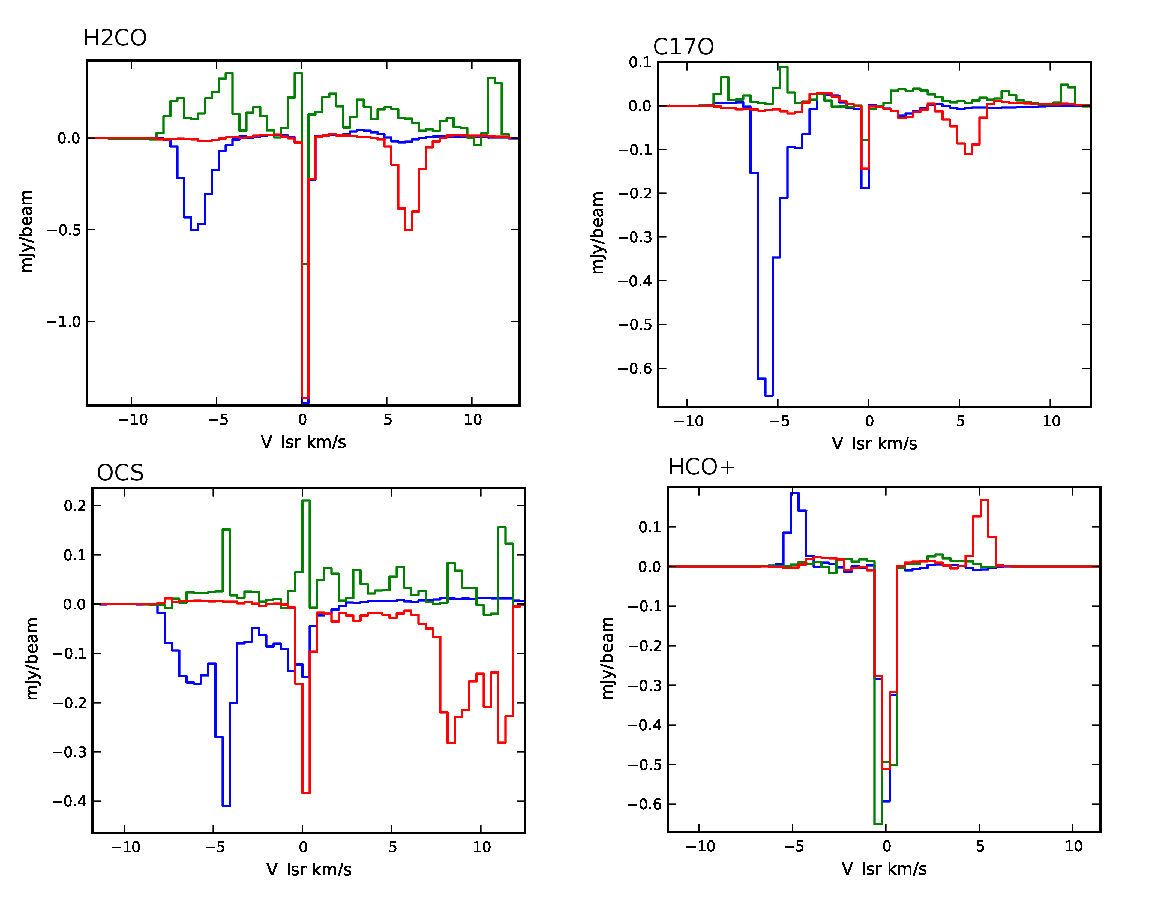
\includegraphics[width=168mm]{Figures/sim/casa_all_spectra.eps}

 \caption{Spectra for each of the simulated species. In each diagram the three spectra are taken from positions on the Y=0 axis, one is at X=0 (green) and the other 2 are from x=$\pm$ N (plus blue, minus red) where N is different for each species. the values for N are: OCS 10AU, H$_2$CO 20AU, C$^{17}$O 28AU, HCO$^+$ 38AU. The locations for these spectra are given in figure \ref{mom0_maps}, the red green and blue curves are taken from the locations marked 1, 2 and 3 respectively.}
 \label{spectra}
\end{figure*}

Figure \ref{spectra} shows spectra from the lines simulated, one from the centre of the image and one on each side of the disc along the Y=0 axis. The most notable thing about these is, despite the fact that the spectra are equally spaced about the centre of the disc, they are not symmetric. Most noticeably in the C$^{17}$O the spectrum from the +X side of the disc is shows significantly more absorption than that of the -X side. In the OCS lines, the two sides are not moving with equal velocities and the line widths and shapes are markedly different. These can be attributed to the non-axissymmetric nature of the model.

\section{Discussion and conclusions} \label{sec:discussion}

In this paper we have presented radiative transfer simulations of a hybrid model comprising a 0.4$\, M_\odot$ self gravitating disc with radius 64$\,AU$ showing spiral density waves, surrounded by an envelope simulated as a collapsing 10$\,M_\odot$ BE-sphere. The main results of these simulations are as follows:\newline

$\bullet$ CASA simulations of this model show that at a distance of 100$\,$pc extraction of kinematic and structural information from continuum and some molecular lines are possible in ALMA band 7.\newline 
$\bullet$ Our simulations show that many molecular species are predominantly seen in absorption against the hot mid-plane of self-gravitating protoplanetary discs, with emission only being seen where voids in the structure of the disc do not provide a bright continuum source to be absorbed.\newline 
$\bullet$ The quiescent nature of the envelope around such discs only obscures lines within $\pm\,$0.5 km$\,$s$^{-1}$ of the systematic velocity.\newline 
$\bullet$ The lines studied (OCS 26$\rightarrow$25, H$_2$CO 4$_{04}$$\rightarrow$3$_{03}$, C$^{17}$O 3$\rightarrow$2 and HCO$^+$ 3$\rightarrow$2) taken together allow all regions of the disc to be sampled and the rotation of the disc to be constrained from the inner edge to the outer edge.\newline 


One assumption made in this model is that the gas and dust are in thermal equilibrium in the disc. If they are not and the dust is significantly cooler than the gas then transitions may not show up in absorption.\newline
The mass of the disc used (0.4$\,\rm{M}_\odot$) is on the high end for early discs (citations for estimate of early class 0 disc masses). Outflows could contaminate measurements of rotation curves meaning that species  which commonly trace outflows, such as CO and HCO$^+$ are not going to be good tracers of disc rotation. However species such as OCS and C$^{17}$O which are not commonly seen in outflows (e.g. van der Tak et al. 2003, Stanke et al. 2007, Yildiz et al 2012, Ren et al. 2011)can be used to trace disc rotation.\newline

We have shown that observations of young, gravitationally-unstable protoplanetary discs can be both seen and differentiated from smooth/stable discs by ALMA. Using a range of molecular lines would allow such observations to be able to determine both the structure and the kinematics of such a disc.

\section*{Acknowledgements}

stuff here
\newpage

\appendix

\section{Grid Construction} \label{sec:gridding} 

In order to construct the grid, candidate points are randomly selected from the volume to be simulated. These candidates then have their density and molecular density compared against a reference point in order to decide if the point is to be used in the grid or not. Candidate grid points are selected at random in cylindrical co-ordinates, linearly spaced in z and $\phi$ and logarithmically spaced in r. For each point to be selected, a random number $\alpha$ is drawn from the semi-open set [0,$\,$1) as a threshold. After selection of random co-ordinates, the hydrogen density and molecular density at the candidate point (n and m, respectively) are compared against the densities of a reference point on the inner edge of the disc (n$_0$ and m$_0$). If $\alpha<\left( \frac{n}{n_0} \right)^{0.3}$ or $\alpha< \left( \frac{m}{m_0} \right)^{0.3}$ then the point is selected for use, otherwise another r, $\phi$, z co-ordinate is selected and this becomes the candidate point. The function comparing the candidate point to the reference point and the candidate point distribution were selected empirically to sample all the scales while ensuring that the majority of points are located in the inner disc where the density is higher. 20\% of these points are forced to be at radii greater than $\sqrt{R_{min}R_{max}}$ (where $R_{min}$ and $R_{max}$ are the inner and outer radius of the model) in order to stop too many of the selected points clustering in the high density disc and leaving the envelope under sampled. In addition to this method of selection, 5\% of the points are linearly distributed in x, y and z with no bias with regards to density or abundance. This provides a minimum level of sampling for the large low density regions in the outer parts of the simulated volume. See figure \ref{points} for an example of the points distribution in r, z. \newline

\begin{figure}
 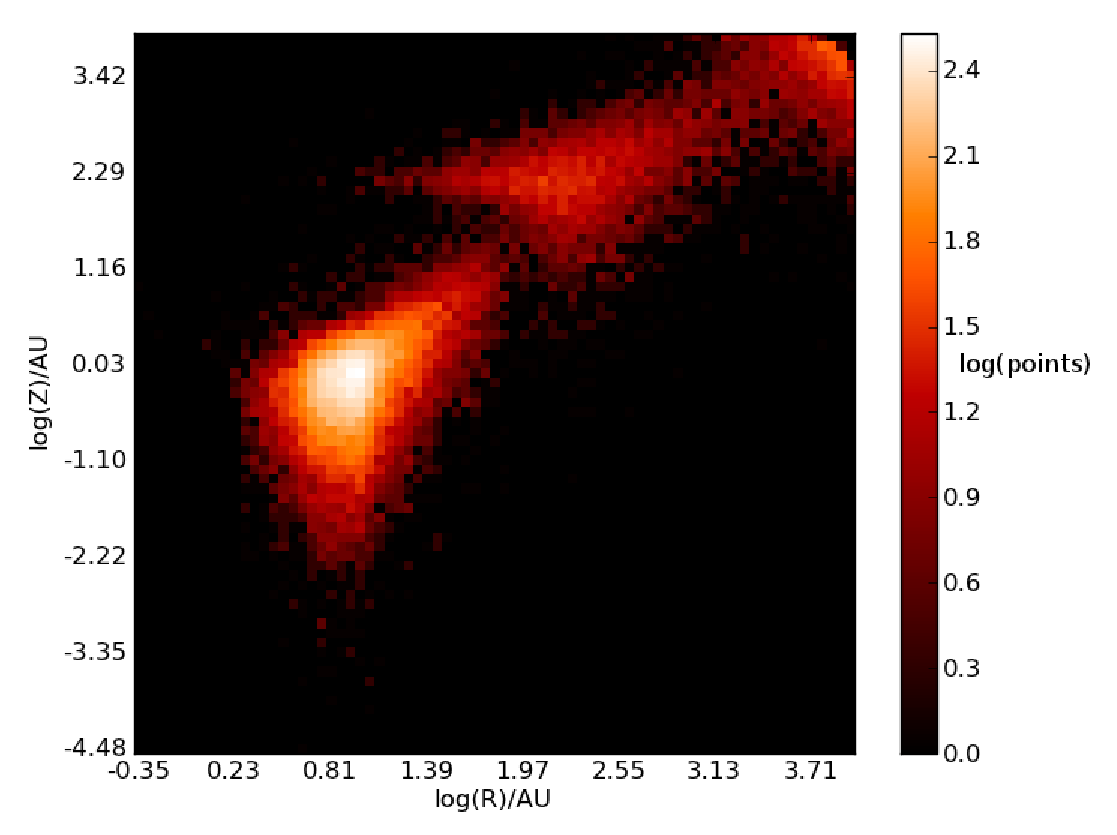
\includegraphics[width=84mm]{Figures/model/lime_points_rz_histo2.eps}
 \caption{A 2D histogram of the point distribution throughout the model. The disc and envelope can be seen as two separate entities which have to be sampled using different point distributions}
 \label{points}
\end{figure}




\section{Other Inclinations} \label{sec:other_inc}

Figures showing different inclinations 
\begin{figure*}
 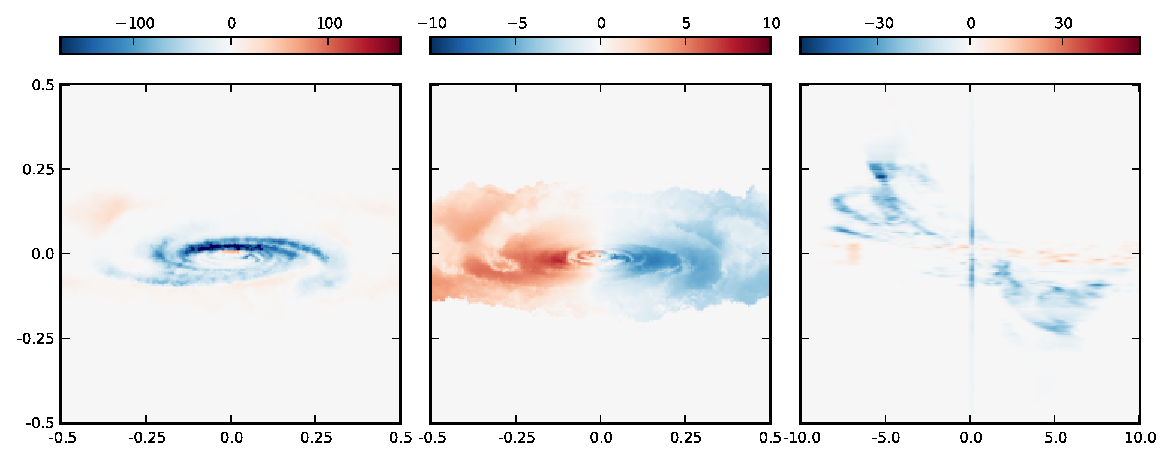
\includegraphics[width=198mm]{Figures/sim/imageC17O_3-2_15deg_all.eps}

 \caption{C$^{17}$O 3-2 15 deg Continuum subtracted mom0}
\end{figure*}

\begin{figure*}
 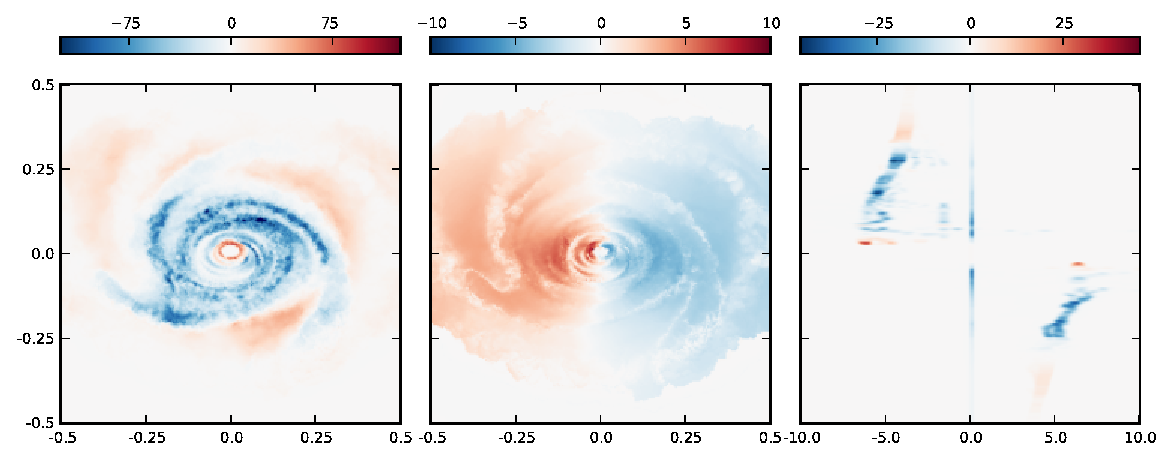
\includegraphics[width=198mm]{Figures/sim/imageC17O_3-2_45deg_all.eps}

 \caption{C$^{17}$O 3-2 45 deg Continuum subtracted mom0}
\end{figure*}

\begin{figure*}
 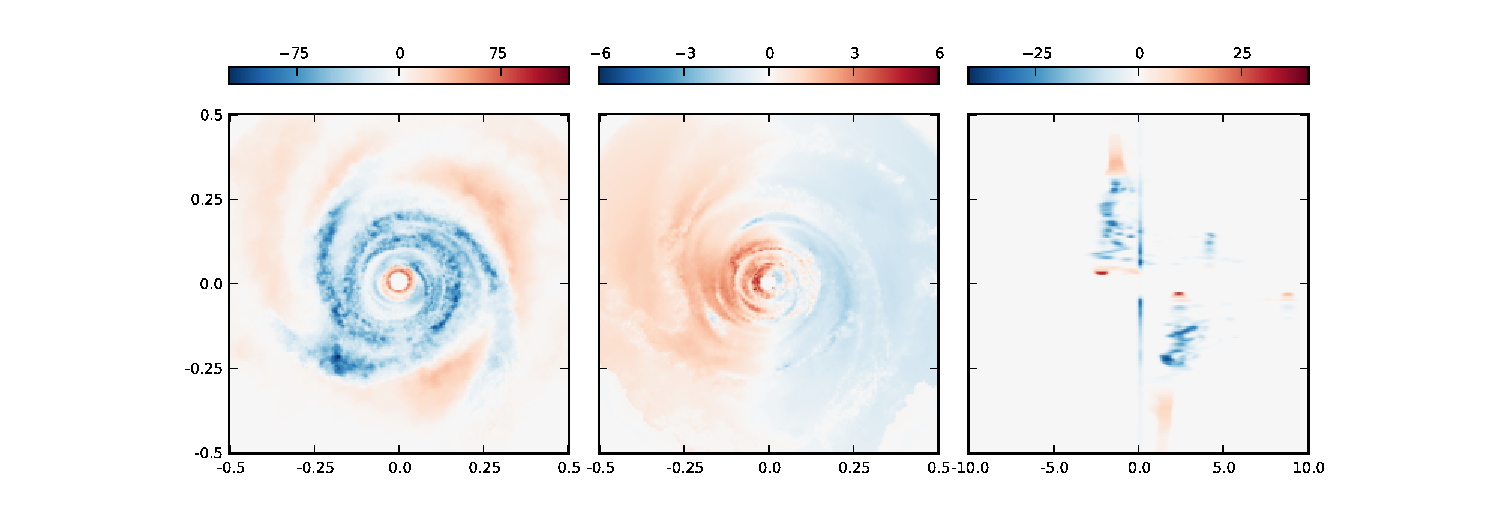
\includegraphics[width=198mm]{Figures/sim/imageC17O_3-2_75deg_all.eps}

 \caption{C$^{17}$O 3-2 75 deg Continuum subtracted mom0}
\end{figure*}

%\begin{figure}
% 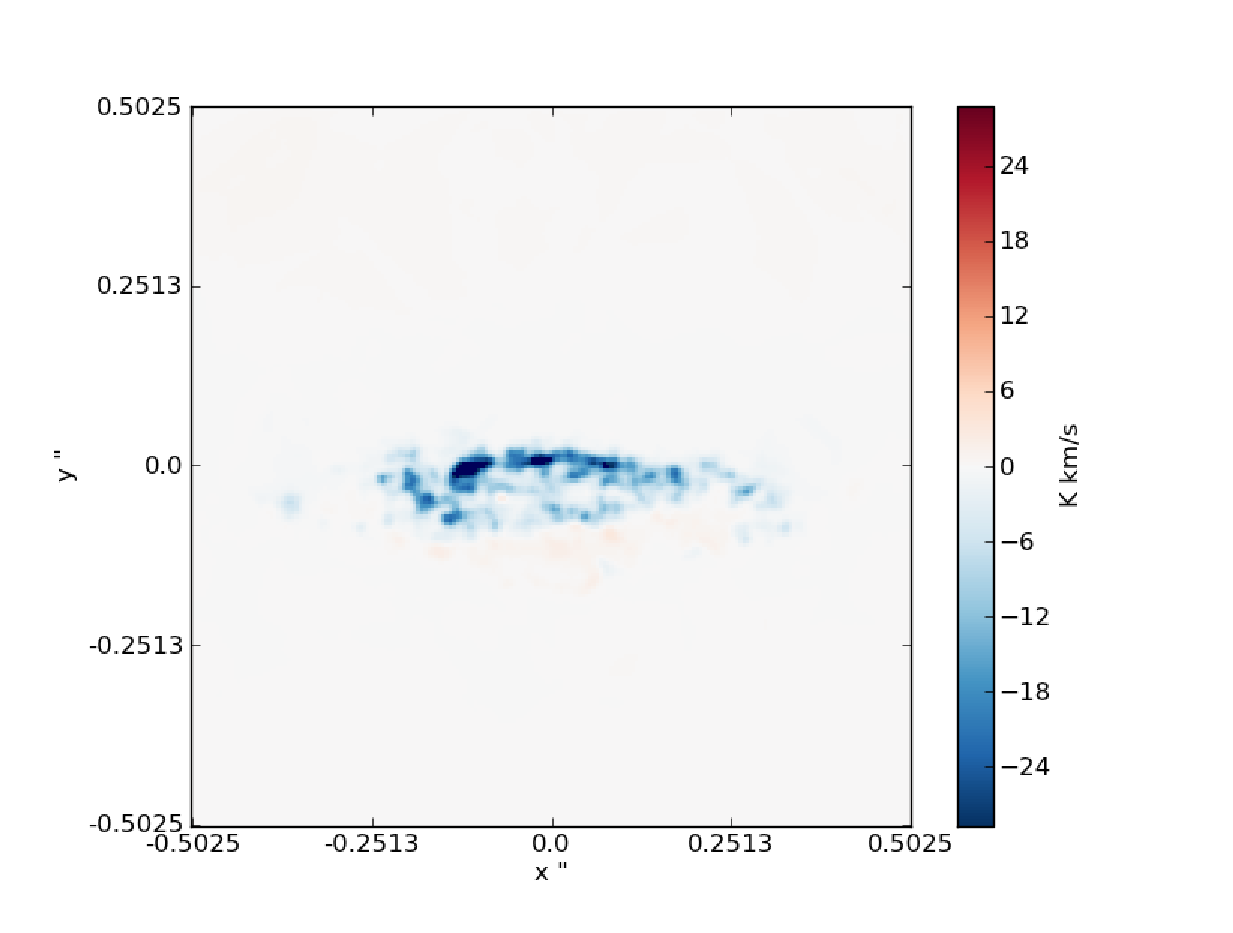
\includegraphics[width=84mm]{Figures/sim/imageC18O_3-2_15deg_contSub.eps}
%
% \caption{C18O 3-2 15 deg Continuum subtracted mom0}
%\end{figure}
%
%%\begin{figure}
%% 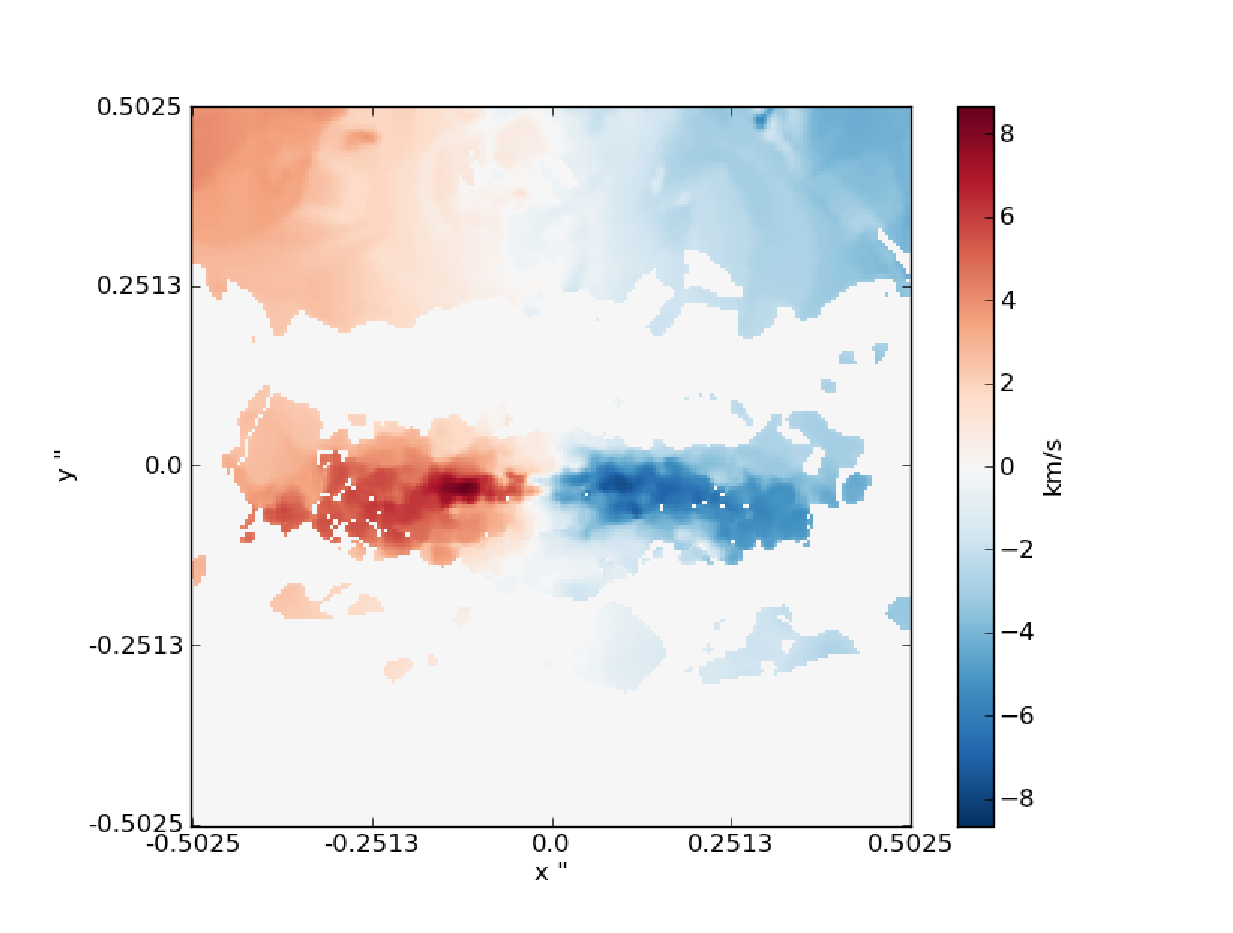
\includegraphics[width=84mm]{Figures/sim/imageC18O_3-2_15deg_mom1.eps}
%%
%% \caption{C18O 3-2 15 deg mom1map}
%%\end{figure}
%
%\begin{figure}
% \includegraphics[width=84mm]{Figures/sim/imageC18O_3-2_15deg_PV_centre.eps}
%
% \caption{C18O 3-2 PV 15 deg through centre}
%\end{figure}
%
%
%\begin{figure}
% 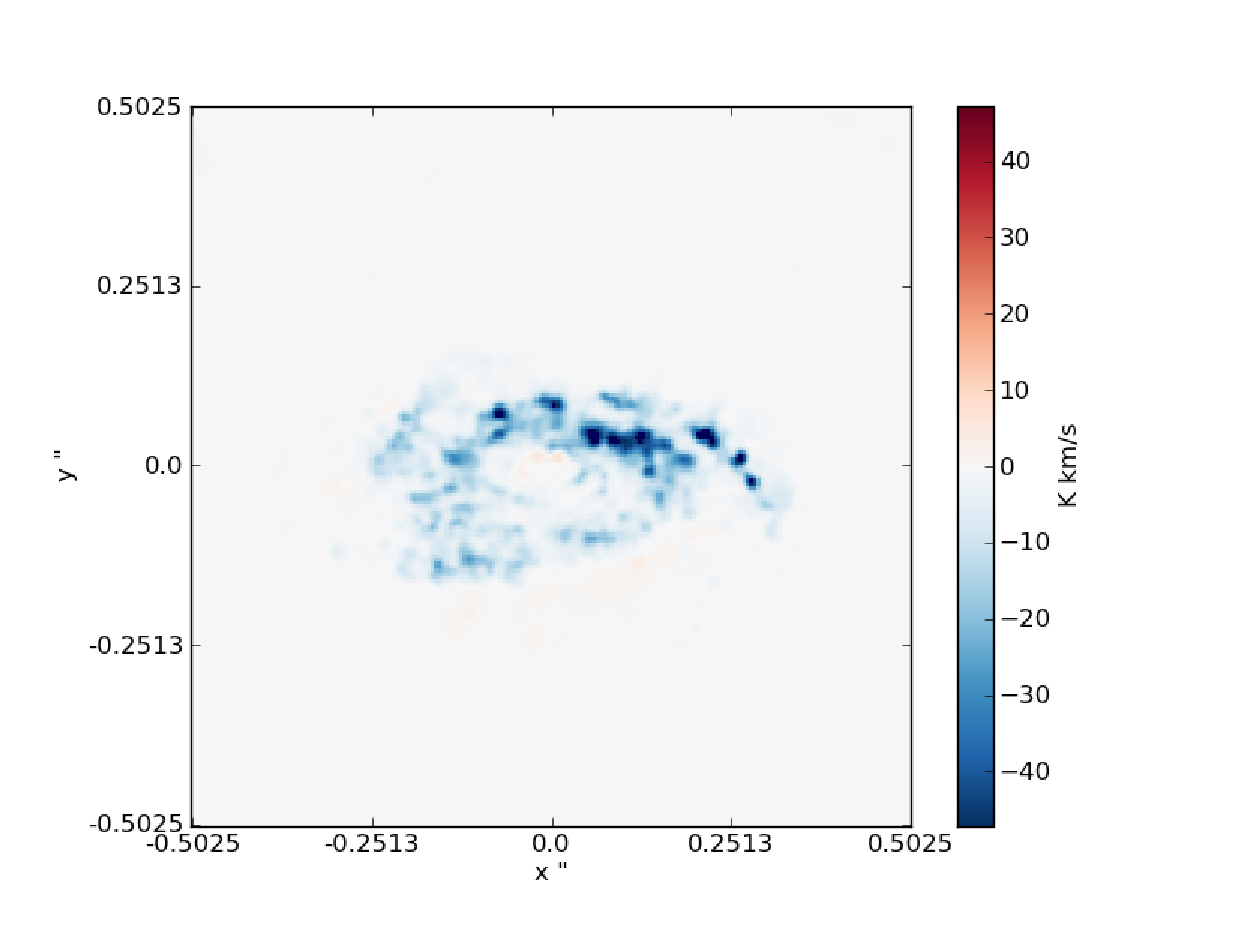
\includegraphics[width=84mm]{Figures/sim/imageC18O_3-2_30deg_contSub.eps}
%
% \caption{C18O 3-2  30 deg Continuum subtracted mom0}
%\end{figure}


%\begin{figure}
% 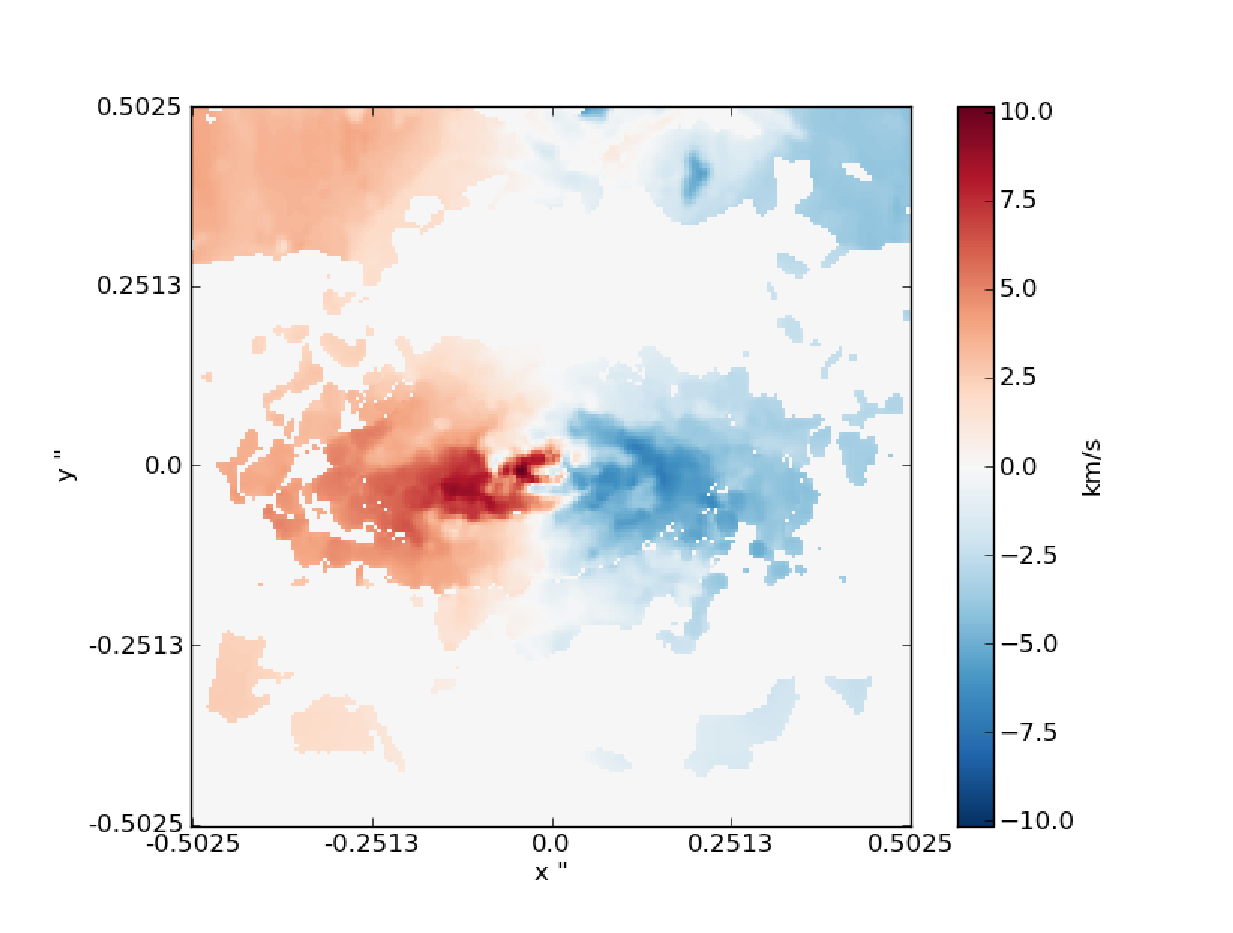
\includegraphics[width=84mm]{Figures/sim/imageC18O_3-2_30deg_mom1.eps}
%
% \caption{C18O 3-2 30 deg mom1map}
%\end{figure}

%\begin{figure}
% \includegraphics[width=84mm]{Figures/sim/imageC18O_3-2_30deg_PV_centre.eps}
%
% \caption{C18O 3-2 30 deg PV through centre}
%\end{figure}
%
%\begin{figure}
% 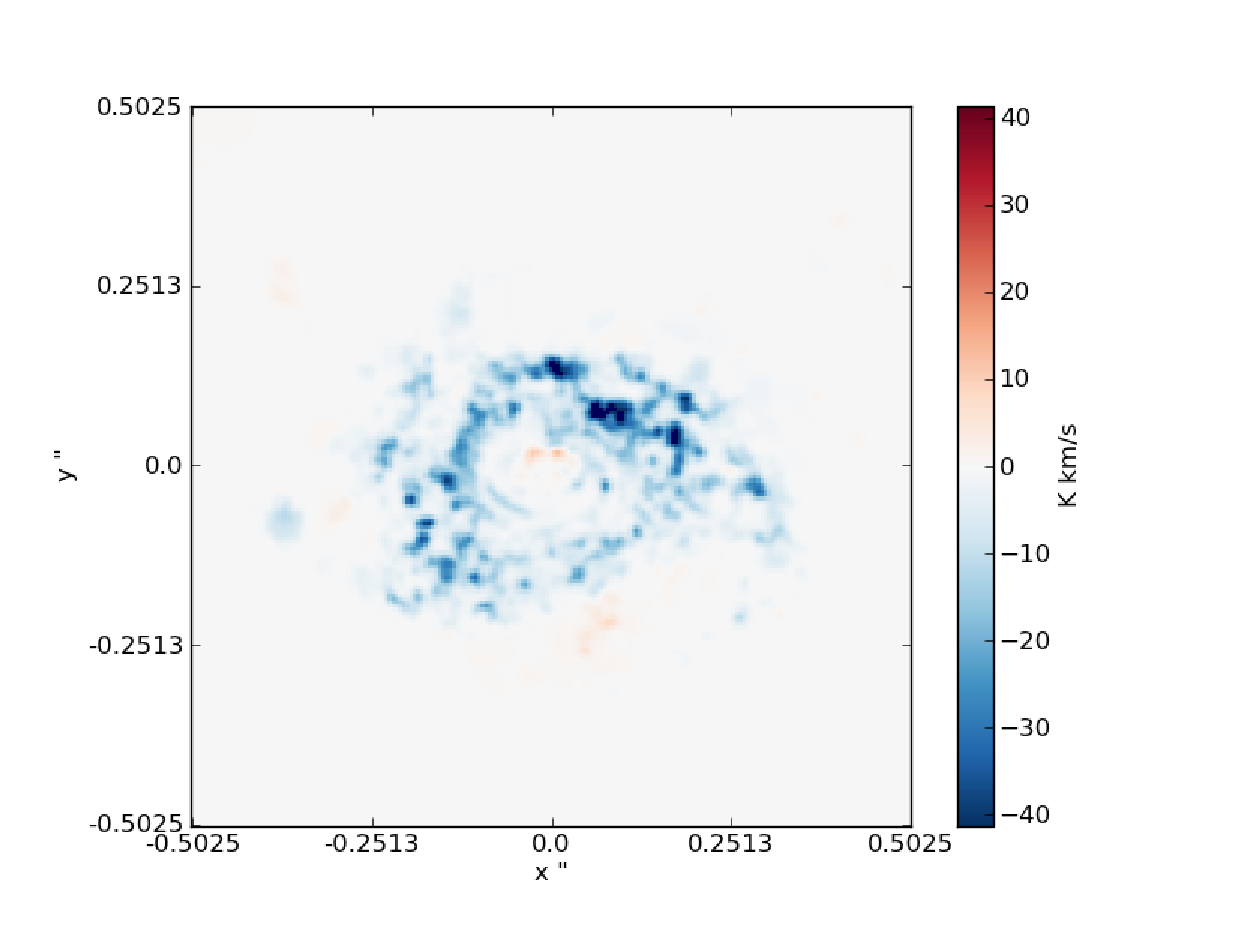
\includegraphics[width=84mm]{Figures/sim/imageC18O_3-2_45deg_contSub.eps}
%
% \caption{C18O 3-2 45 deg Continuum subtracted mom0}
%\end{figure}
%
%%\begin{figure}
%% 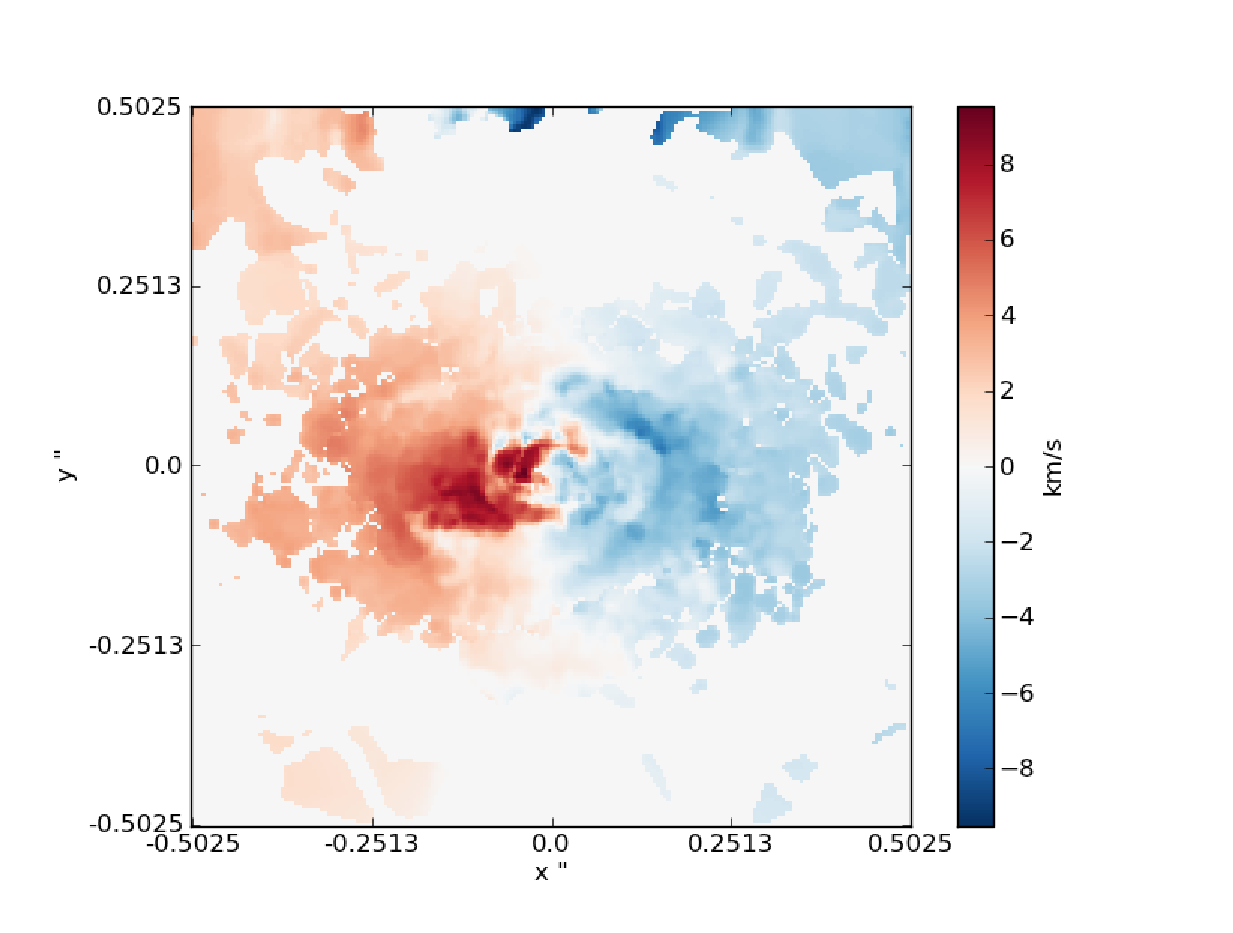
\includegraphics[width=84mm]{Figures/sim/imageC18O_3-2_45deg_mom1.eps}
%%
%% \caption{C18O 3-2 45 deg mom1map}
%%\end{figure}
%
%\begin{figure}
% \includegraphics[width=84mm]{Figures/sim/imageC18O_3-2_45deg_PV_centre.eps}
%
% \caption{C18O 3-2 45 deg PV through centre}
%\end{figure}
%
%
%\begin{figure}
% \includegraphics[width=84mm]{Figures/sim/imageC18O_3-2_60deg_contSub.eps}
%
% \caption{C18O 3-2 60 deg Continuum subtracted mom0}
%\end{figure}
%
%%\begin{figure}
%% 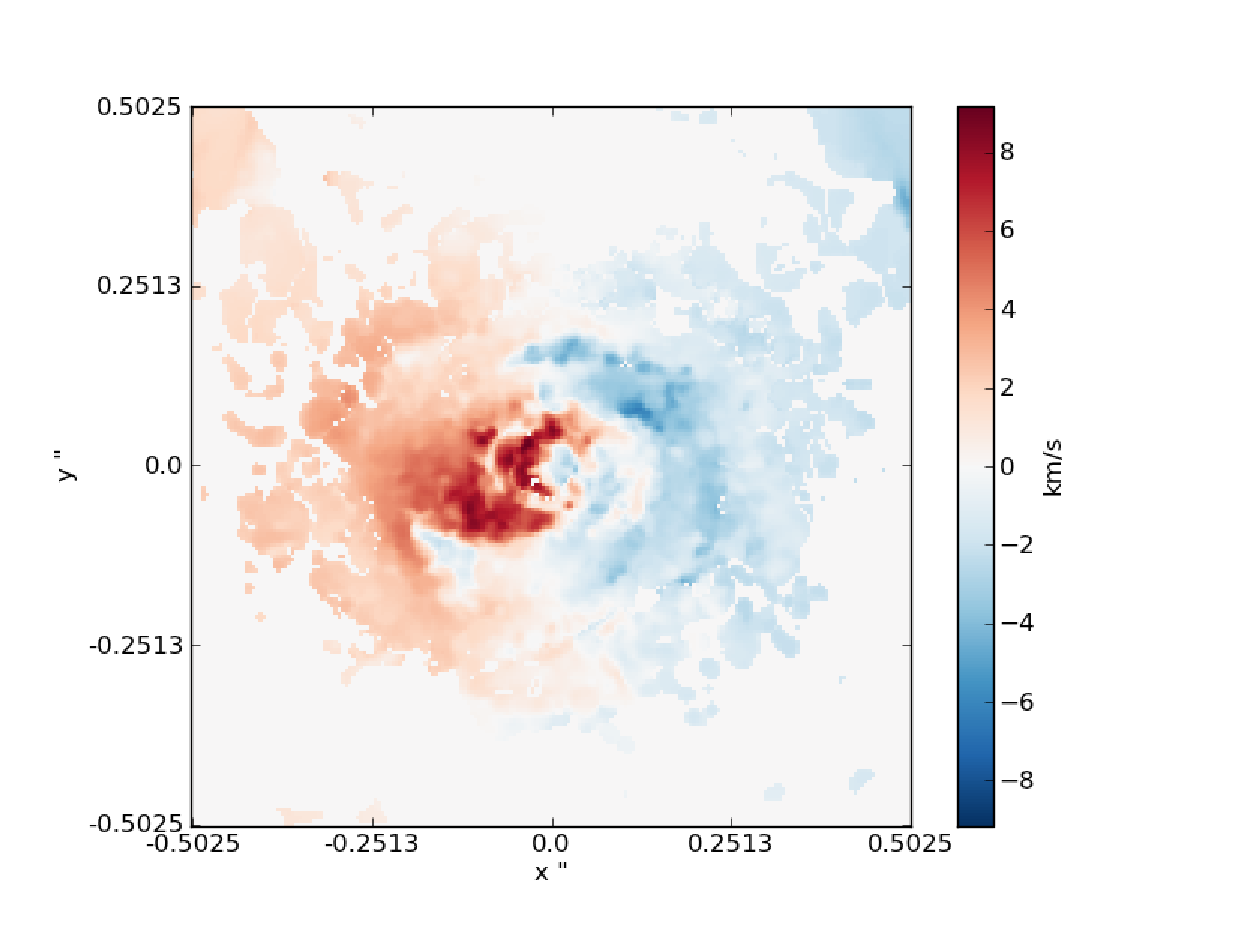
\includegraphics[width=84mm]{Figures/sim/imageC18O_3-2_60deg_mom1.eps}
%%
%% \caption{C18O 3-2 60 deg mom1map}
%%\end{figure}
%
%\begin{figure}
% 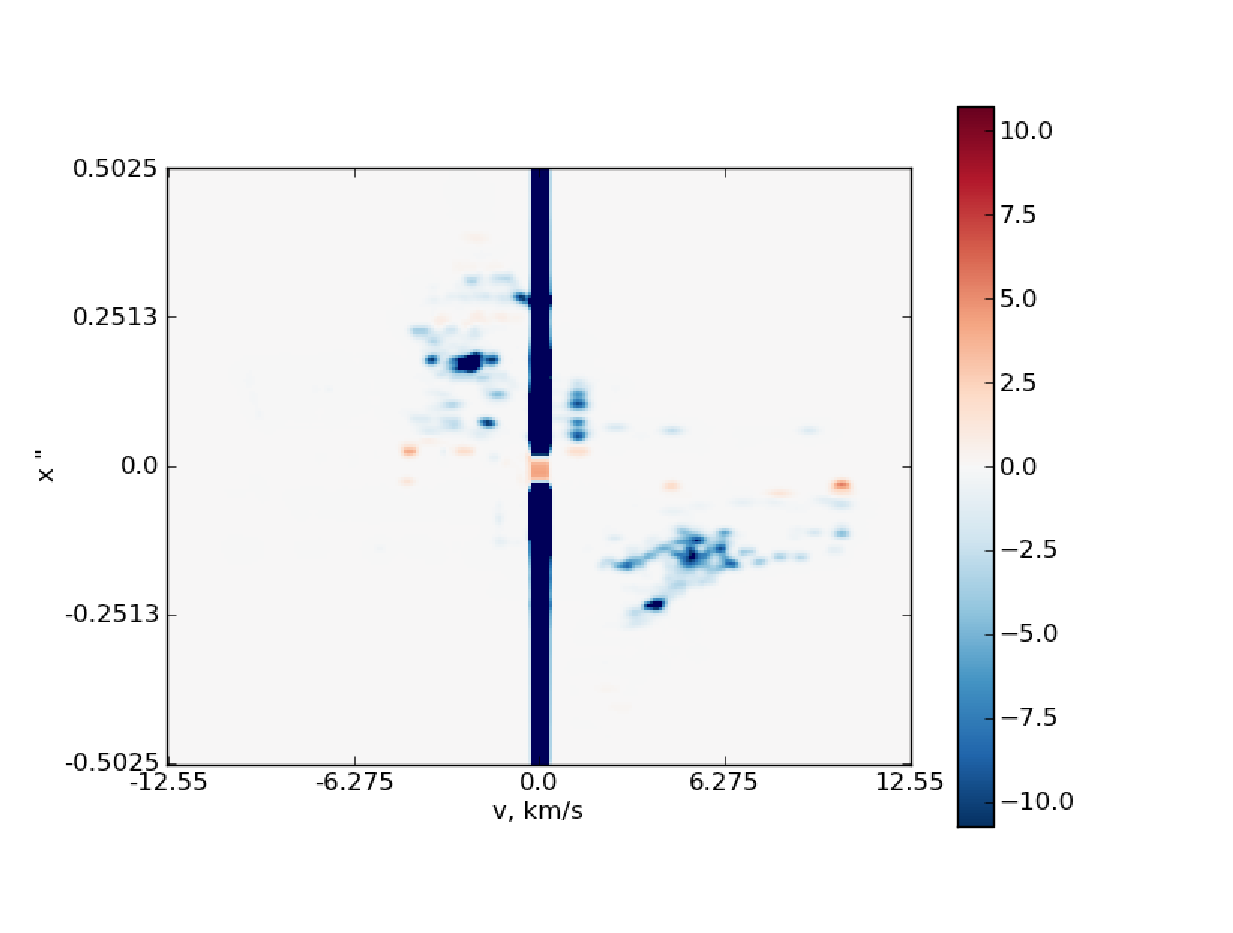
\includegraphics[width=84mm]{Figures/sim/imageC18O_3-2_60deg_PV_centre.eps}
%
% \caption{C18O 3-2 60 deg PV through centre}
%\end{figure}
%
%\begin{figure}
% 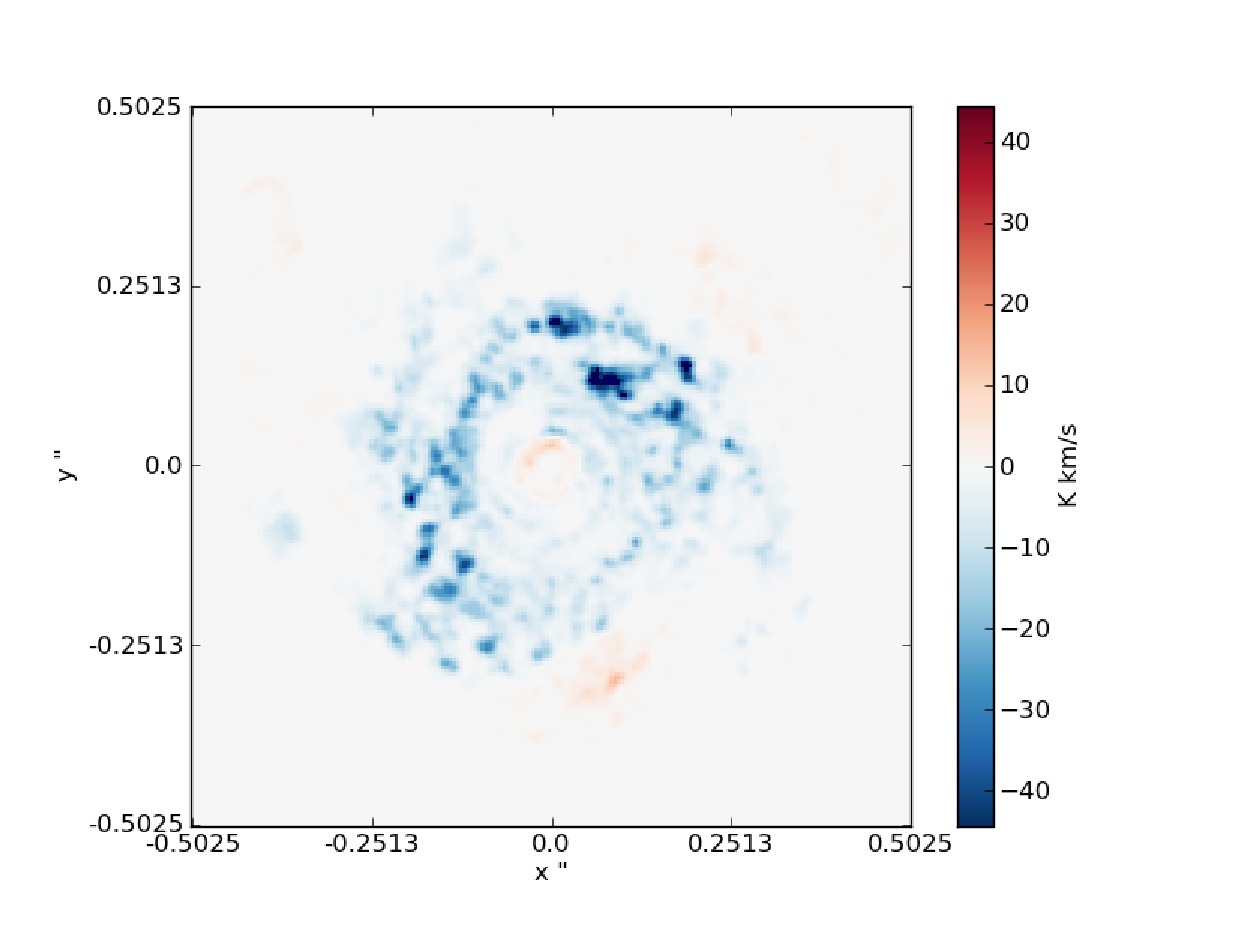
\includegraphics[width=84mm]{Figures/sim/imageC18O_3-2_75deg_contSub.eps}
%
% \caption{C18O 3-2 75 deg Continuum subtracted mom0}
%\end{figure}
%
%%\begin{figure}
%% 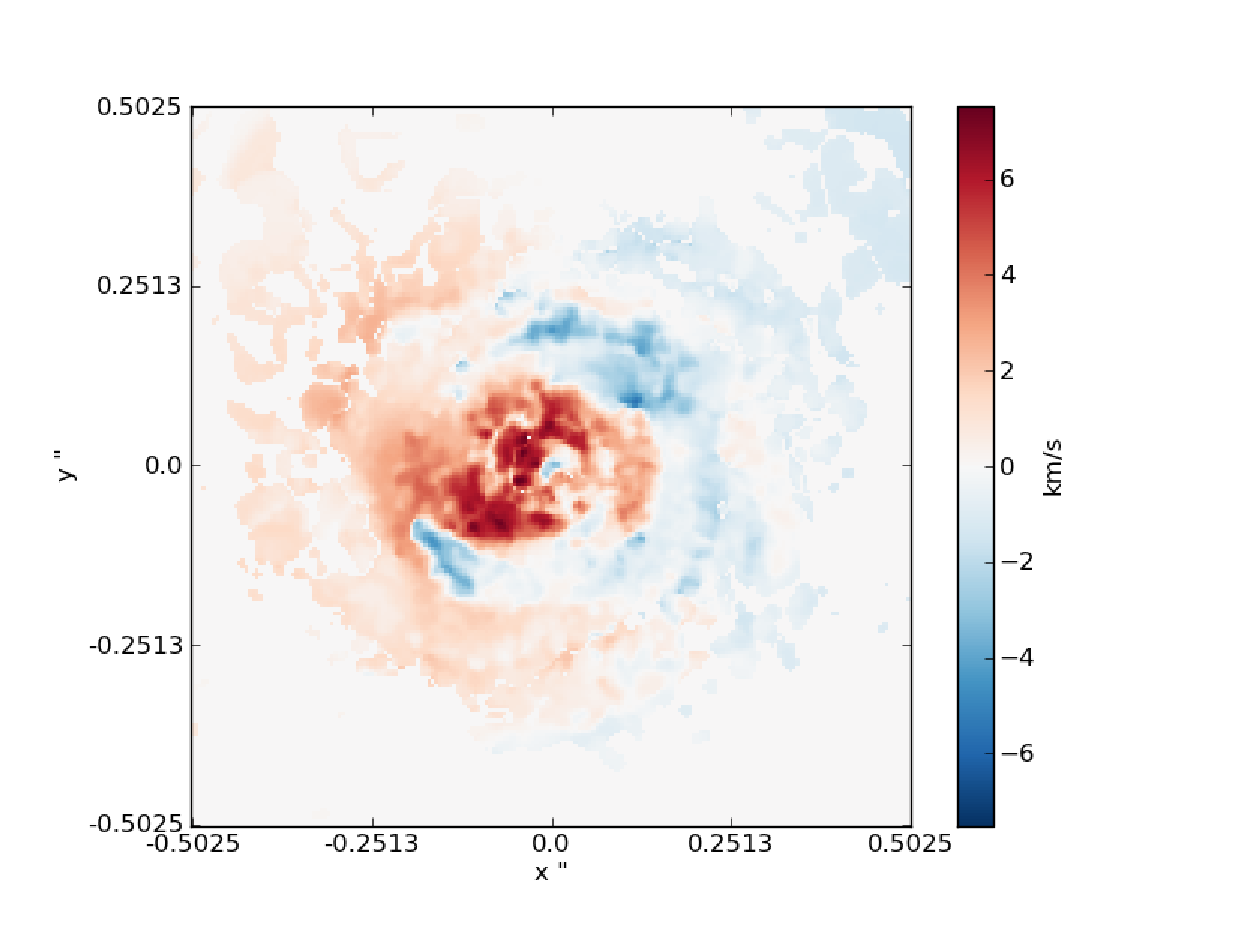
\includegraphics[width=84mm]{Figures/sim/imageC18O_3-2_75deg_mom1.eps}
%%
%% \caption{C18O 3-2 75 deg mom1map}
%%\end{figure}
%
%\begin{figure}
%%  \showthe\columnwidth % Use this to determine the width of the figure.
%  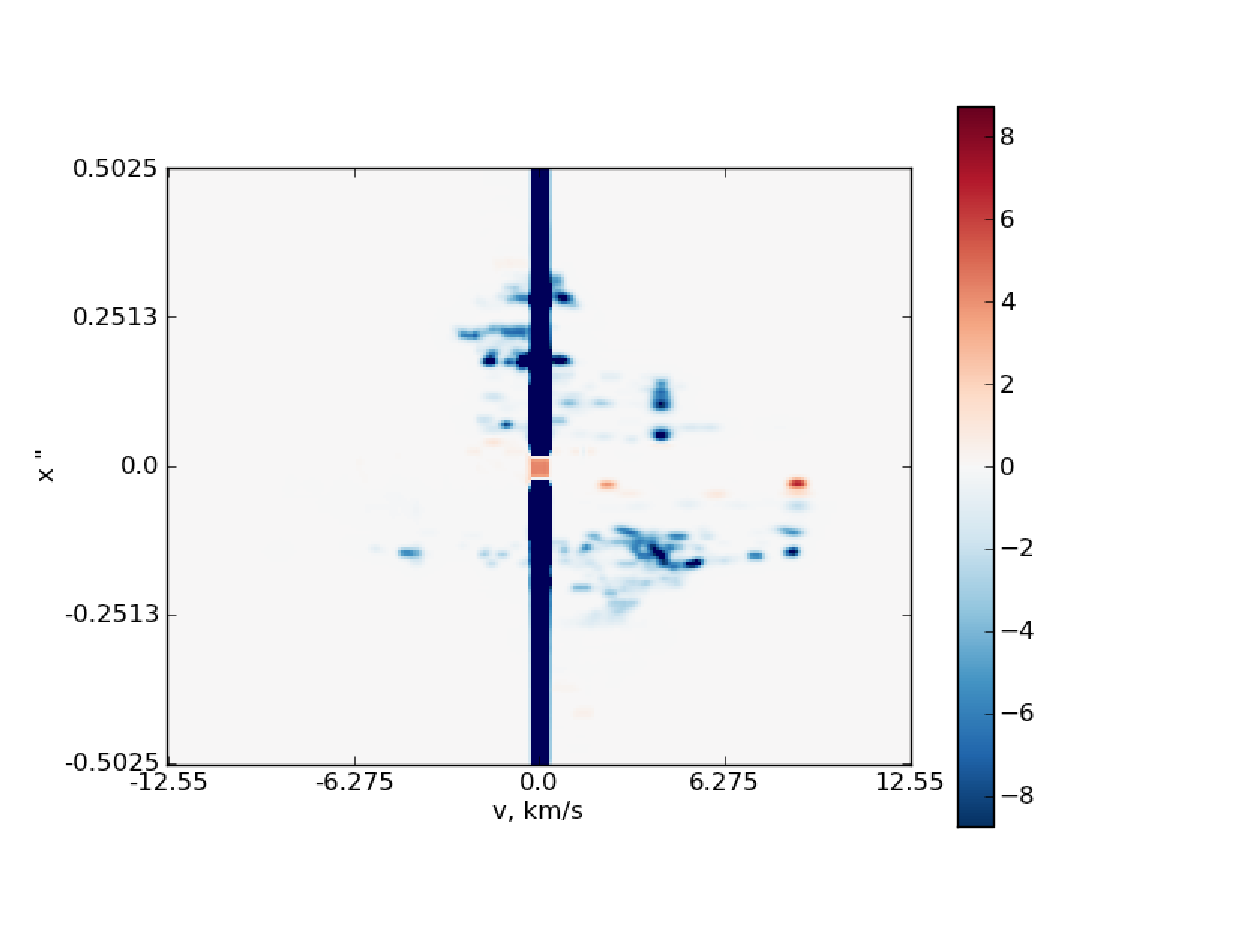
\includegraphics[width=84mm]{Figures/sim/imageC18O_3-2_75deg_PV_centre.eps}
%  \caption{C18O 3-2 75 deg PV through centre}
%\end{figure}

\bsp
%
\label{lastpage}
%
\end{document}
